\chapter{\IfLanguageName{dutch}{Resultaten}{Results}}%
\label{ch:resultaten}

Dit hoofdstuk presenteert de resultaten van de verschillende testcases die uitgevoerd zijn. Bij elke analyse worden zowel de resultaten ten opzichte van de baseline als de onderlinge verschillen tussen de nieuwe cloud-oplossingen met elkaar vergeleken. Eerst wordt belicht wat de huidige toepassing als uitslag gaf en wordt dit als nulmeting gezien voor verdere vergelijkingen. Daarna volgt een analyse van prestaties van de toepassingen in de meest gunstige omstandigheden. Vervolgens komt een bespreking van de output bij de minst gunstige omstandigheden, de cold start. Hier op volgend wordt de focus gelegd op hoe de omgevingen anticipeerden bij een stresstest om de elasticiteit in kaart te brengen. Tot slot volgt een kostenraming voor de verwerking van 100 verzoeken op een maand. Na dit onderdeel is alle informatie aanwezig om een doordachte conclusie te formuleren.

\section{Baseline: De Huidige Architectuur}

Om een idee te krijgen van hoe de huidige toepassing reageert in een een gunstige en ongunstige omstandigheid, werd dit nagebootst door een sequentiële aanroep met of zonder interval. De huidige toepassing draait op een productie-omgeving en daarom werd er gekozen om slechts 10 aanroepen te doen om het systeem niet te lang en te zwaar te belasten. Dit moet voldoende zijn om aan te tonen dat er een probleem is bij een piekbelasting.

\subsection{Verwerking met Interval}

Bij een interval van 6 minuten werd verzekerd dat de vorige verwerking afgelopen was, zodat er geen \textit{resources} gedeeld moeten worden over meerdere processen.

\begin{figure}[H]
    \centering
    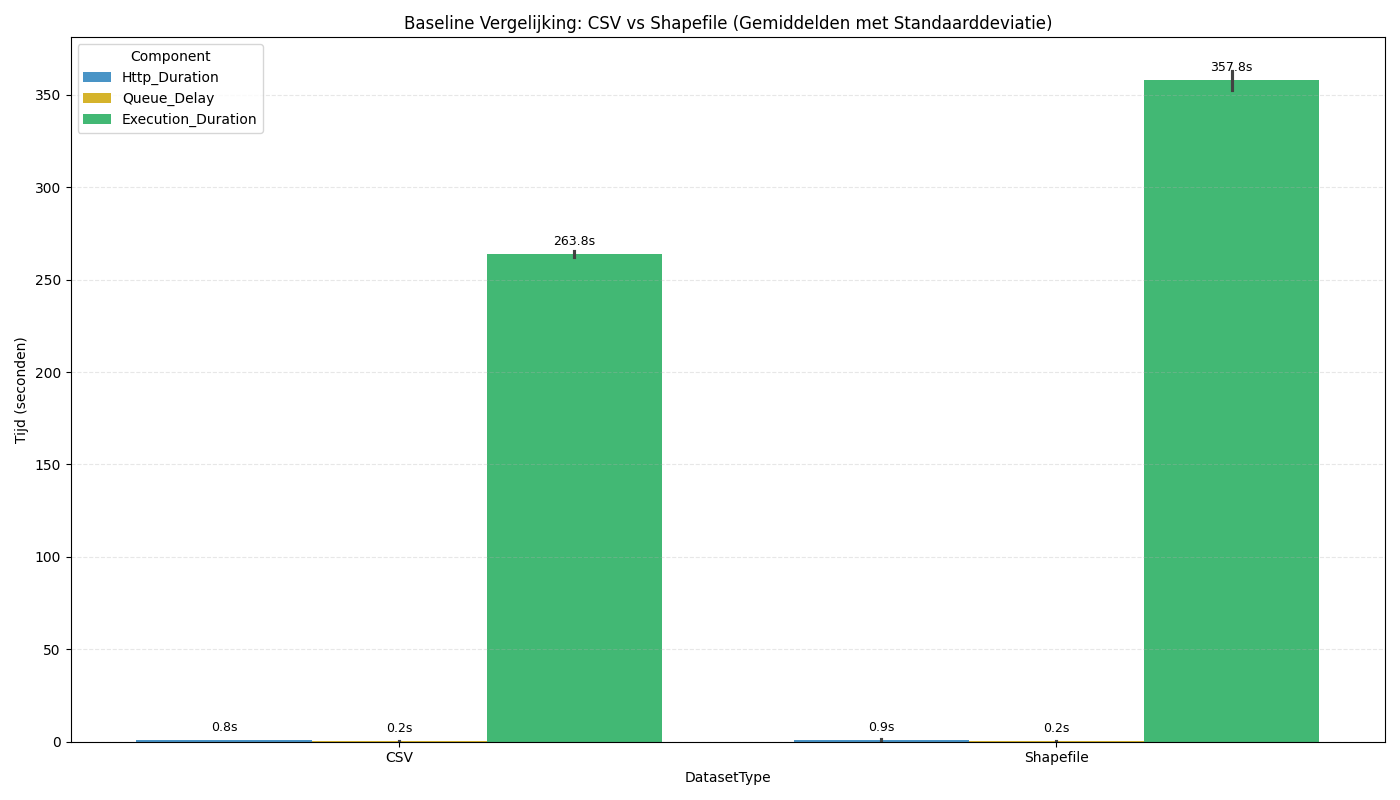
\includegraphics[width=\textwidth]{../graphics/azure_function_sequentieel_interval_barplot_csv_shapefile.png}
    \caption{Baseline Vergelijking: CSV vs Shapefile (Gemiddelden met Standaarddeviatie)}
\end{figure}

Uit deze grafiek wordt duidelijk dat er een verschil is in de gemiddelde verwerkingstijd van datasets met CSV als bestandstype ten opzichte van Shapefile als type. Aangezien de aanvraagtijd en wachtrijvertraging in beide gevallen kort zijn, geeft dit aan dat het verschil zit in de logica van de verwerking tussen beide types en dat het niet aan de infrastructuur ligt. De standaarddeviatie is voor beide types ook klein. Dit geeft aan dat de verwerkingstijd van de meeste aanvragen dicht bij het gemiddelde liggen, waardoor geconcludeerd kan worden dat de verwerkingstijden in dit scenario constant zijn. 

\subsection{Verwerking zonder Interval}

Zonder interval moet het systeem reageren op aanvragen binnen dezelfde tijdspanne wat de druk op de infrastructuur vergroot. Vandaar dat de testrun zonder interval aanzien wordt als de test in ongunstige omstandigheden.
\\
\\
Bij de sequentiële test zonder interval werd de aanvraag altijd correct ontvangen, maar faalde de verwerking meerdere keren door een \textit{race condition}. Omdat herhaaldelijk dezelfde dataset werd opgevraagd, blokkeerde een parallel proces de toegang tot het resultaatbestand. Hoewel dit scenario in de praktijk zelden voorkomt bij individuele aanvragen, legt deze testcase een fundamenteel conflict bloot in de huidige afhandeling van gedeelde resources. Dit probleem is in de nieuwe toepassingen verholpen.

\begin{figure}[H]
    \centering
    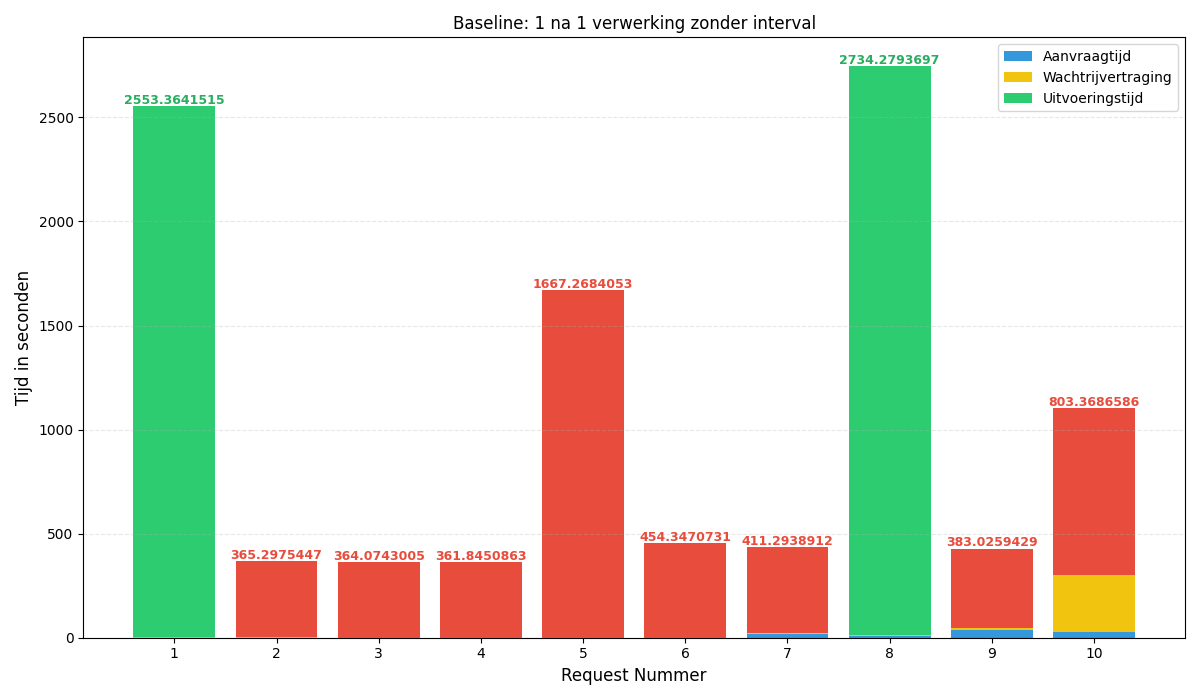
\includegraphics[width=\textwidth]{../graphics/azure_function_sequentieel_zonder_interval_stack_bar.png}
    \caption{Baseline: 1 na 1 verwerking zonder interval}
\end{figure}

Wat eerst opvalt in de grafiek zijn de rode balken die staan voor een verwerking met error. Dit laat duidelijk zien dat 80\% van de verwerkingen in de \textit{QueueTrigger} faalden. Enkel de verwerking van een dataset na aanvraag 1 en 8 zijn gelukt. De verwerkingstijd van deze 2 geslaagde processen zijn wel opvallend lang met respectievelijk 2553 en 2734 seconden. 
\\
\\
Ook opmerkelijk zijn de verwerkingstijden van run 5 en 10 die ondanks het falen toch aan de hoge kant zijn. Bij run 10 is er ook een wachtrijvertraging die er uitspringt tegenover de andere verwerkingen.
\\
\\
\begin{figure}
    \centering
    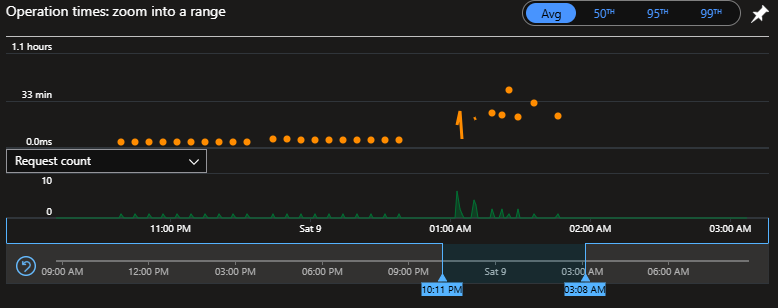
\includegraphics[width=\textwidth]{../graphics/screenshot_app_insights_zonder_interval.png}
    \caption{Screenshot van de grafiek in Applications Insight van testruns Azure Function op productie}
\end{figure}

Bij het onderzoeken van de verwerkingen in de productie-omgeving in verband met de testruns zonder interval kwam naar voor dat er naast de initiële \textit{QueueTrigger}-processen die aangevraagd waren via een HTTP-call dat er nog andere processen opgestart waren door \textit{retries}. Hierbij werden ook lange verwerkingstijden geregistreerd. Dit is te zien in de screenshot hierboven, alsook is duidelijk te zien dat het systeem meer tijd nodig had in het algemeen bij de testrun zonder interval ten opzichte van de testrun met interval.
\\
\\
Deze resultaten bevestigen de bewering van Agromanager dat zij prestatieproblemen ondervinden bij een piekbelasting, waardoor de verwerking van datasets heel lang duren. 

\section{Warm Start: Gunstige Omstandigheden}

In dit scenario werd gekeken naar de prestaties van de containers wanneer ze niet naar 0 geschaald waren en instant konden reageren op verzoeken. Er wordt een onderscheid gemaakt tussen CSV en Shapefile als bestandstypes bij de vergelijkingen.

\subsection{Aanvraagtijd}

\begin{figure}[H]
    \centering
    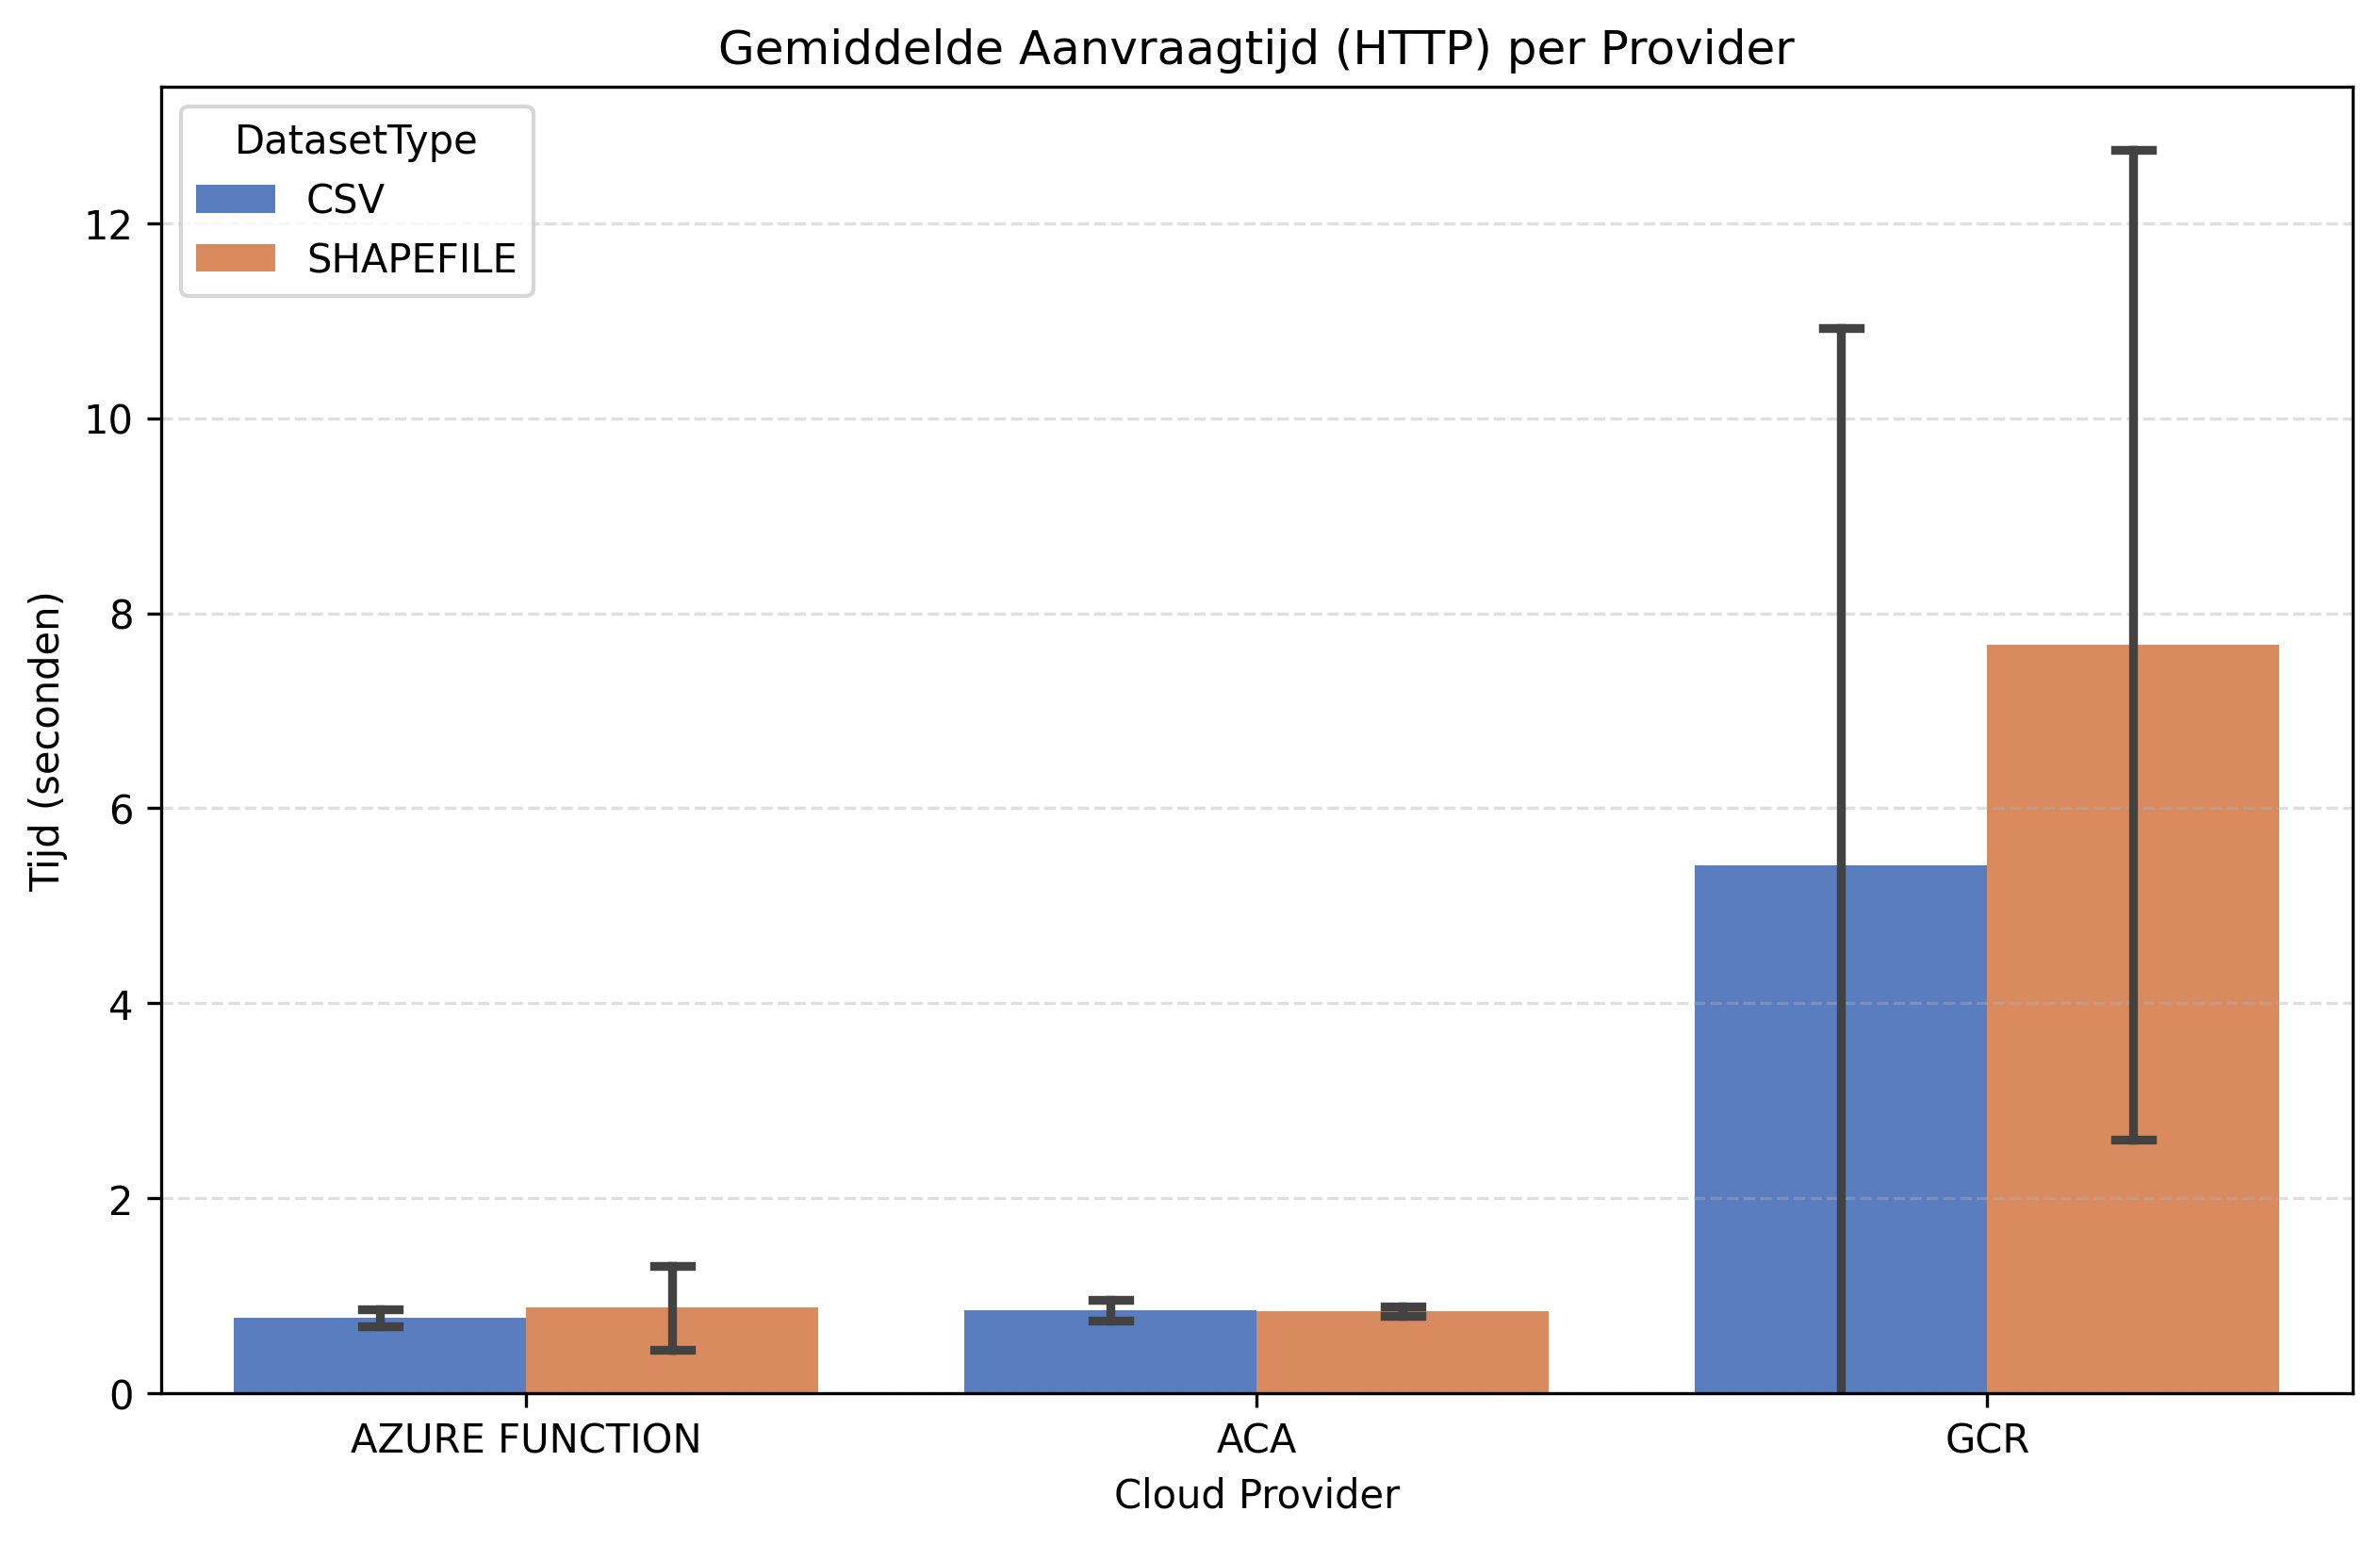
\includegraphics[width=\textwidth]{../graphics/warmstart_plotbar_http.png}
    \caption{Plotbar: Gemiddelde aanvraagtijd (HTTP) per provider}
\end{figure}

Uit de grafiek wordt er afgeleid dat GCR gemiddeld trager reageerde bij de afhandeling van de aanvragen ten opzichte van de Azure Function en ACA. Zowel voor CSV als voor Shapefile. Daarentegen valt op dat Azure Function en ACA gelijkaardige aanvraagtijden hanteren. 

\begin{figure}[H]
    \centering
    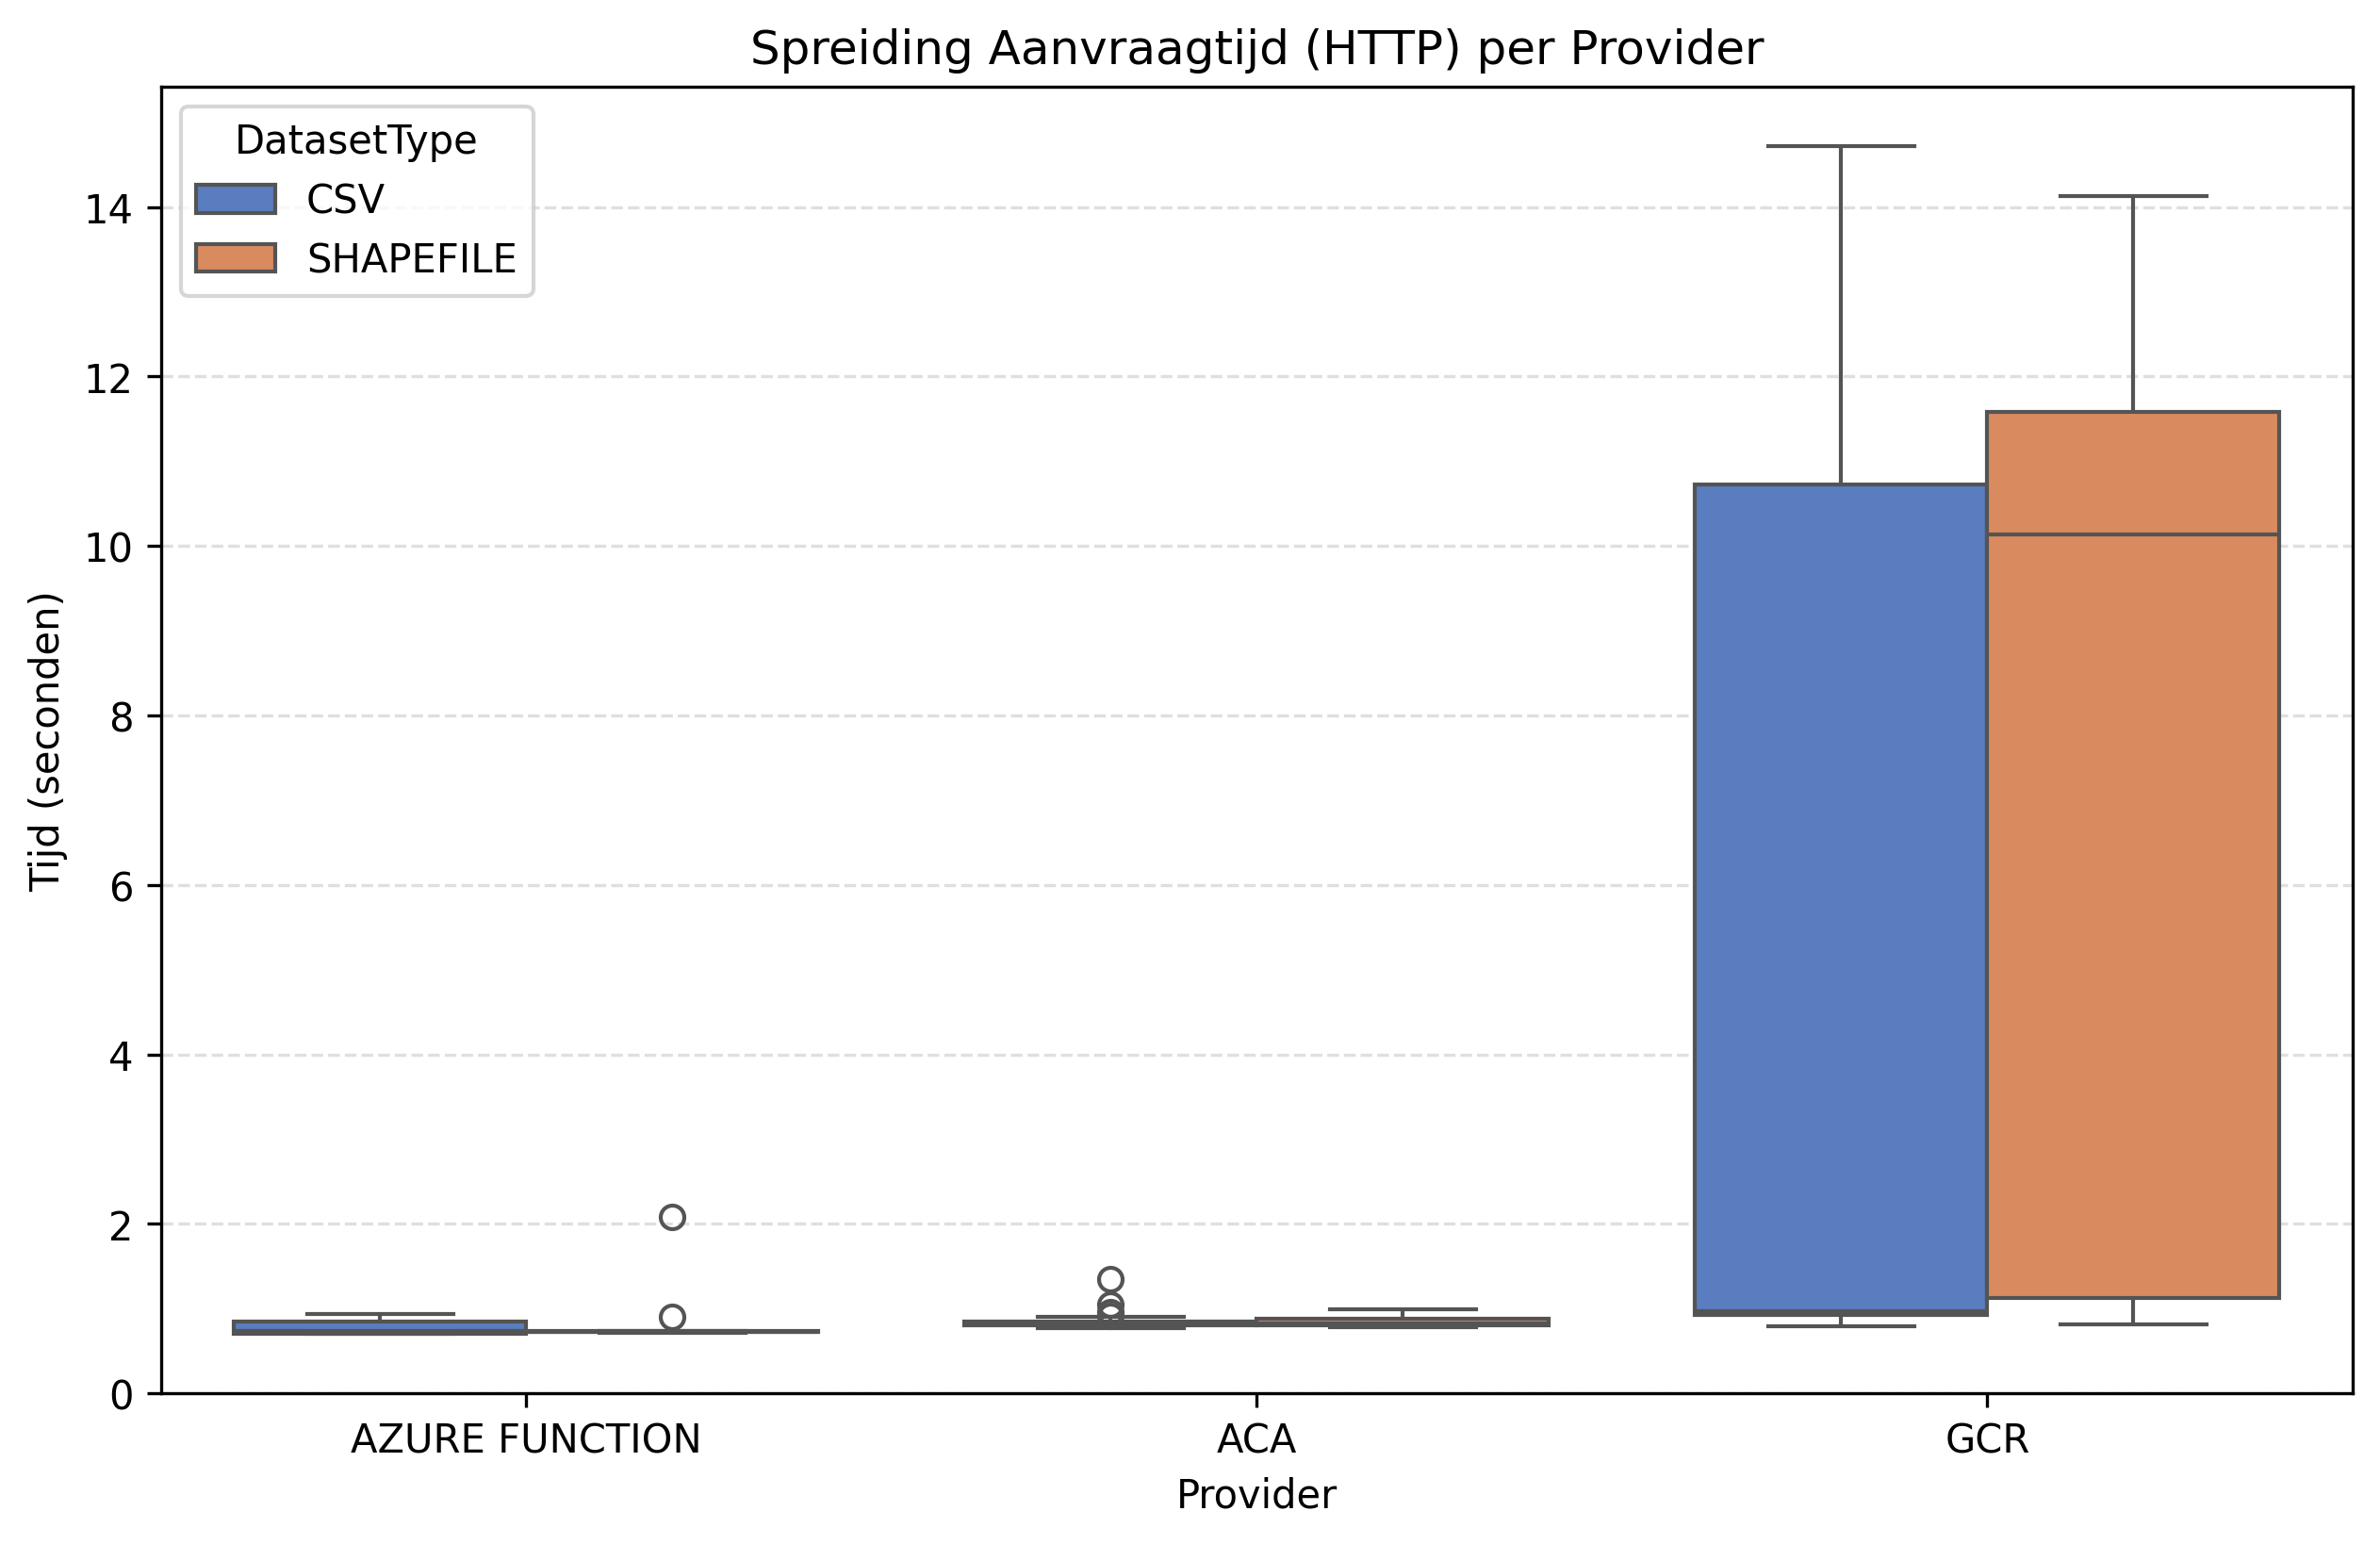
\includegraphics[width=\textwidth]{../graphics/warmstart_plotbox_http.png}
    \caption{Plotbox: Spreiding aanvraagtijd (HTTP) per provider}
\end{figure}

Deze kaart met de spreidingen van aanvragen bevestigt wat er in de vorige grafiek bij GCR als standaardeviatie getoond werd. De aanvragen worden voor de beide types op een inconsistente manier verwerkt. Azure Function en ACA tonen een consistente verwerking.

\subsubsection{Hypothese H1}

\begin{description}
    \item[Stelling:] De overhead van het netwerk is voor de nieuwe cloud-oplossingen hetzelfde als voor de bestaande toepassing. 
    \item[Resultaat:] Verworpen ($p < 0,001$)
\end{description}

Hoewel de nulmeting (0,83s) en ACA (0,85s) ongeveer dezelfde prestaties leveren, vertoont GCR (6,55s) een opvallende vertraging. De huidige toepassing en ACA zijn hier superieur.

\subsection{Wachtrijvertraging}

\begin{figure}[H]
    \centering
    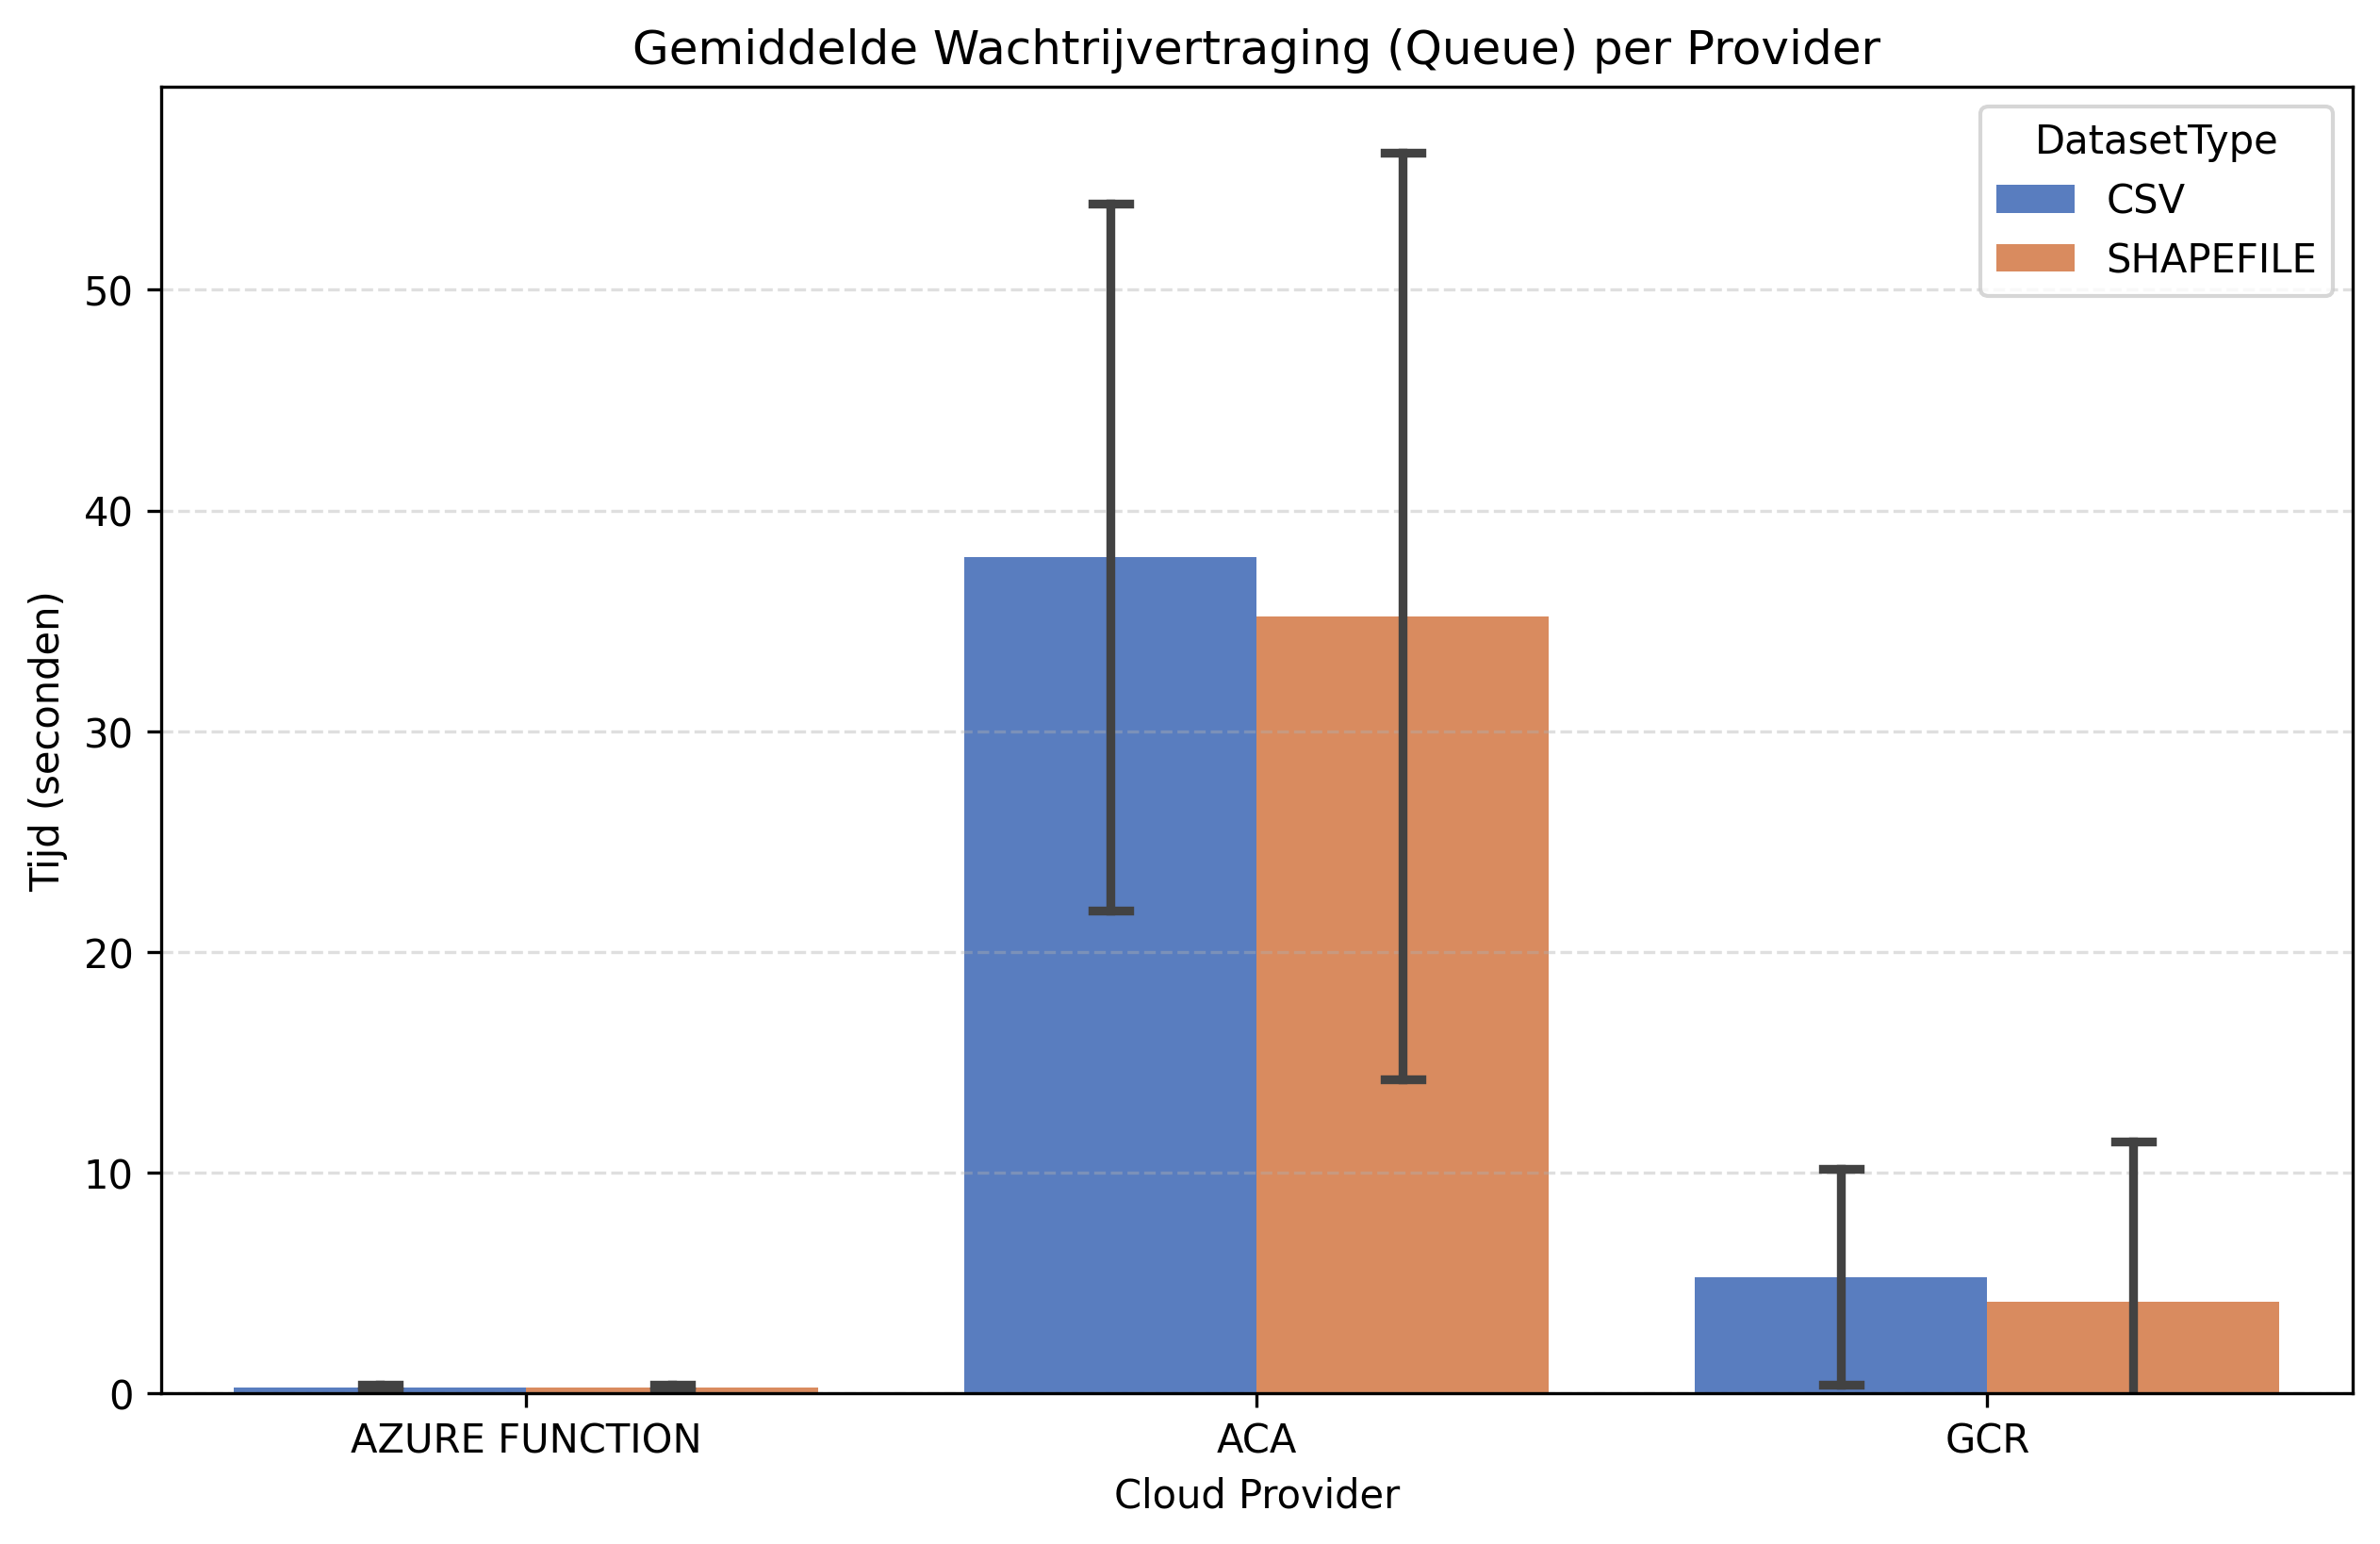
\includegraphics[width=\textwidth]{../graphics/warmstart_plotbar_queue.png}
    \caption{Plotbar: Gemiddelde wachtrijvertraging (Queue) per Provider}
\end{figure}

\begin{figure}[H]
    \centering
    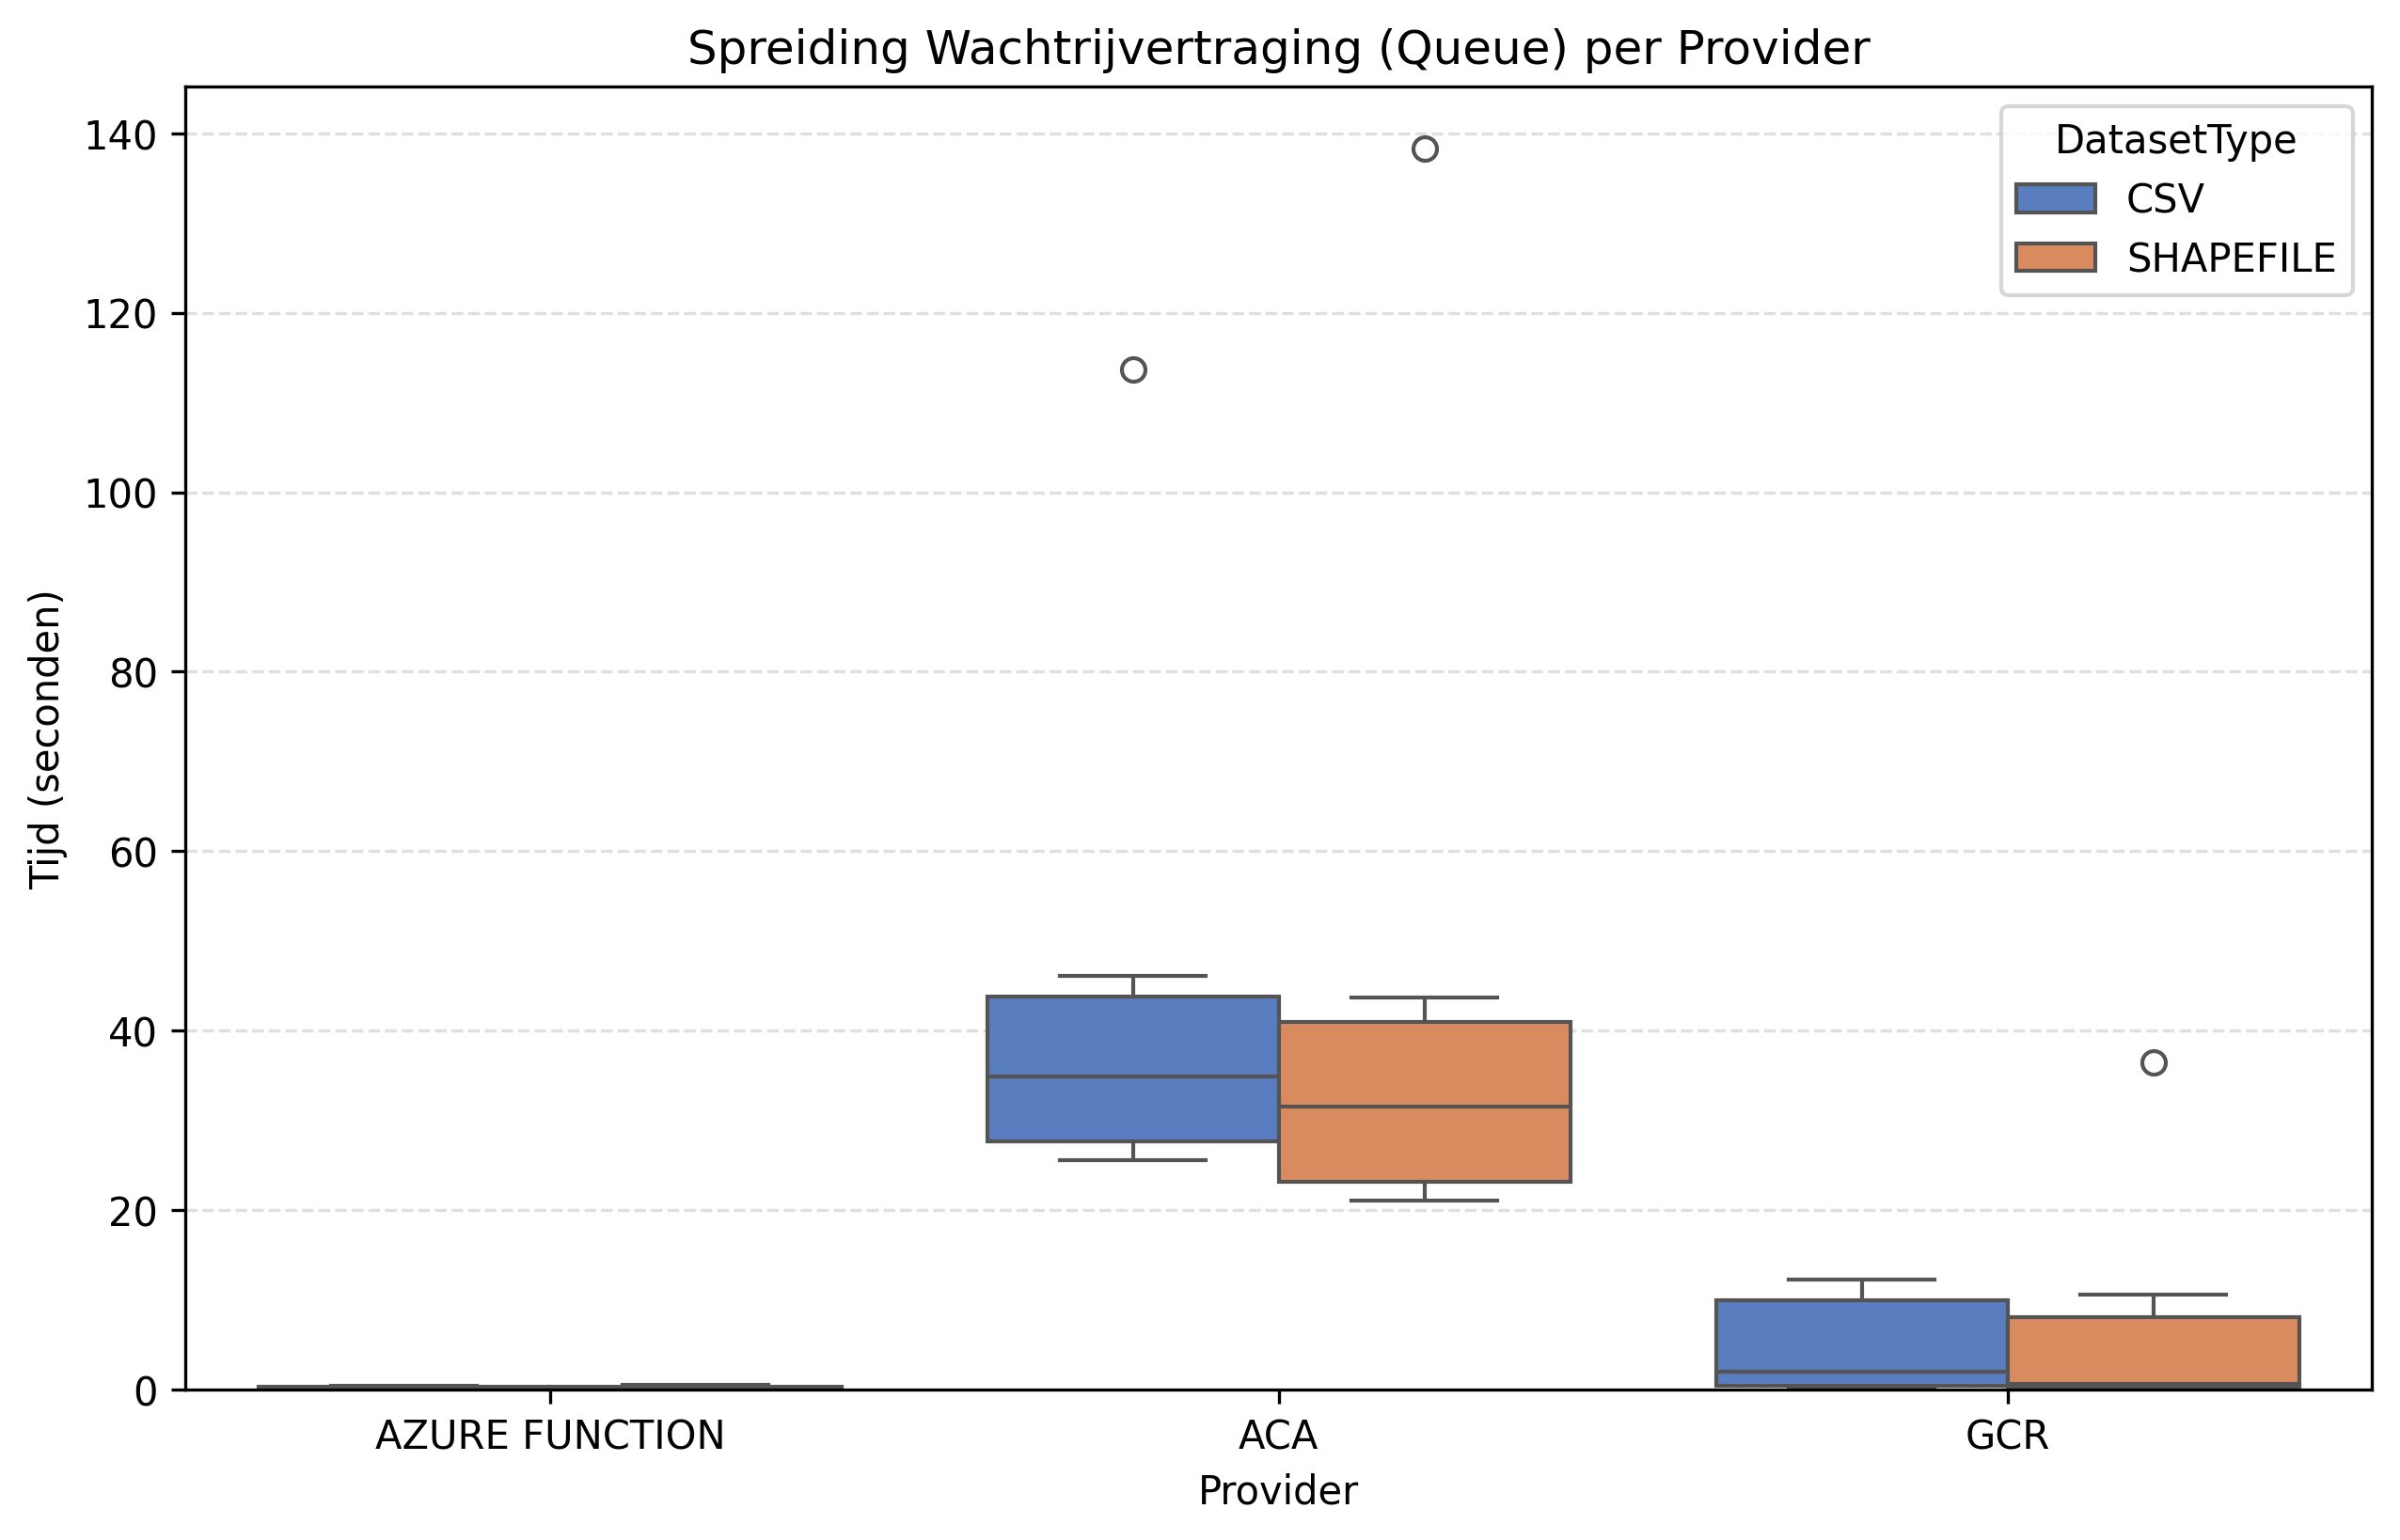
\includegraphics[width=\textwidth]{../graphics/warmstart_plotbox_queue.png}
    \caption{Plotbox: Spreiding wachtrijvertraging (Queue) per provider}
\end{figure}

Er valt een groot verschil op tussen ACA en de andere omgevingen. De standaarddeviatie van dit platform duidt hier ook een grote spreiding van de gemiddelde wachtrijvertragingen aan. GCR komt dichter in de buurt van de bestaande Azure Function, maar geeft ook een grotere spreiding en vertraging aan. Nog opmerkelijk is dat Shapefile minder vertraging ondervond bij ACA en GCR ten opzichte van CSV.

\subsubsection{Hypothese H2}

\begin{description}
    \item[Stelling:] Er is geen verschil tussen GCR en ACA in de tijd die nodig is om een container aan een job toe te wijzen. 
    \item[Resultaat:] Verworpen ($p < 0,001$)
\end{description}

GCR (4,71s) scoort veel beter dan ACA (36,56s) bij het toewijzen van een container aan het bericht. Dit betekent dat de orchestrator van Google Cloud Run veel efficiënter is, dan de orchestrator van Azure Container Apps.

\subsection{Verwerkingstijd}

\begin{figure}[H]
    \centering
    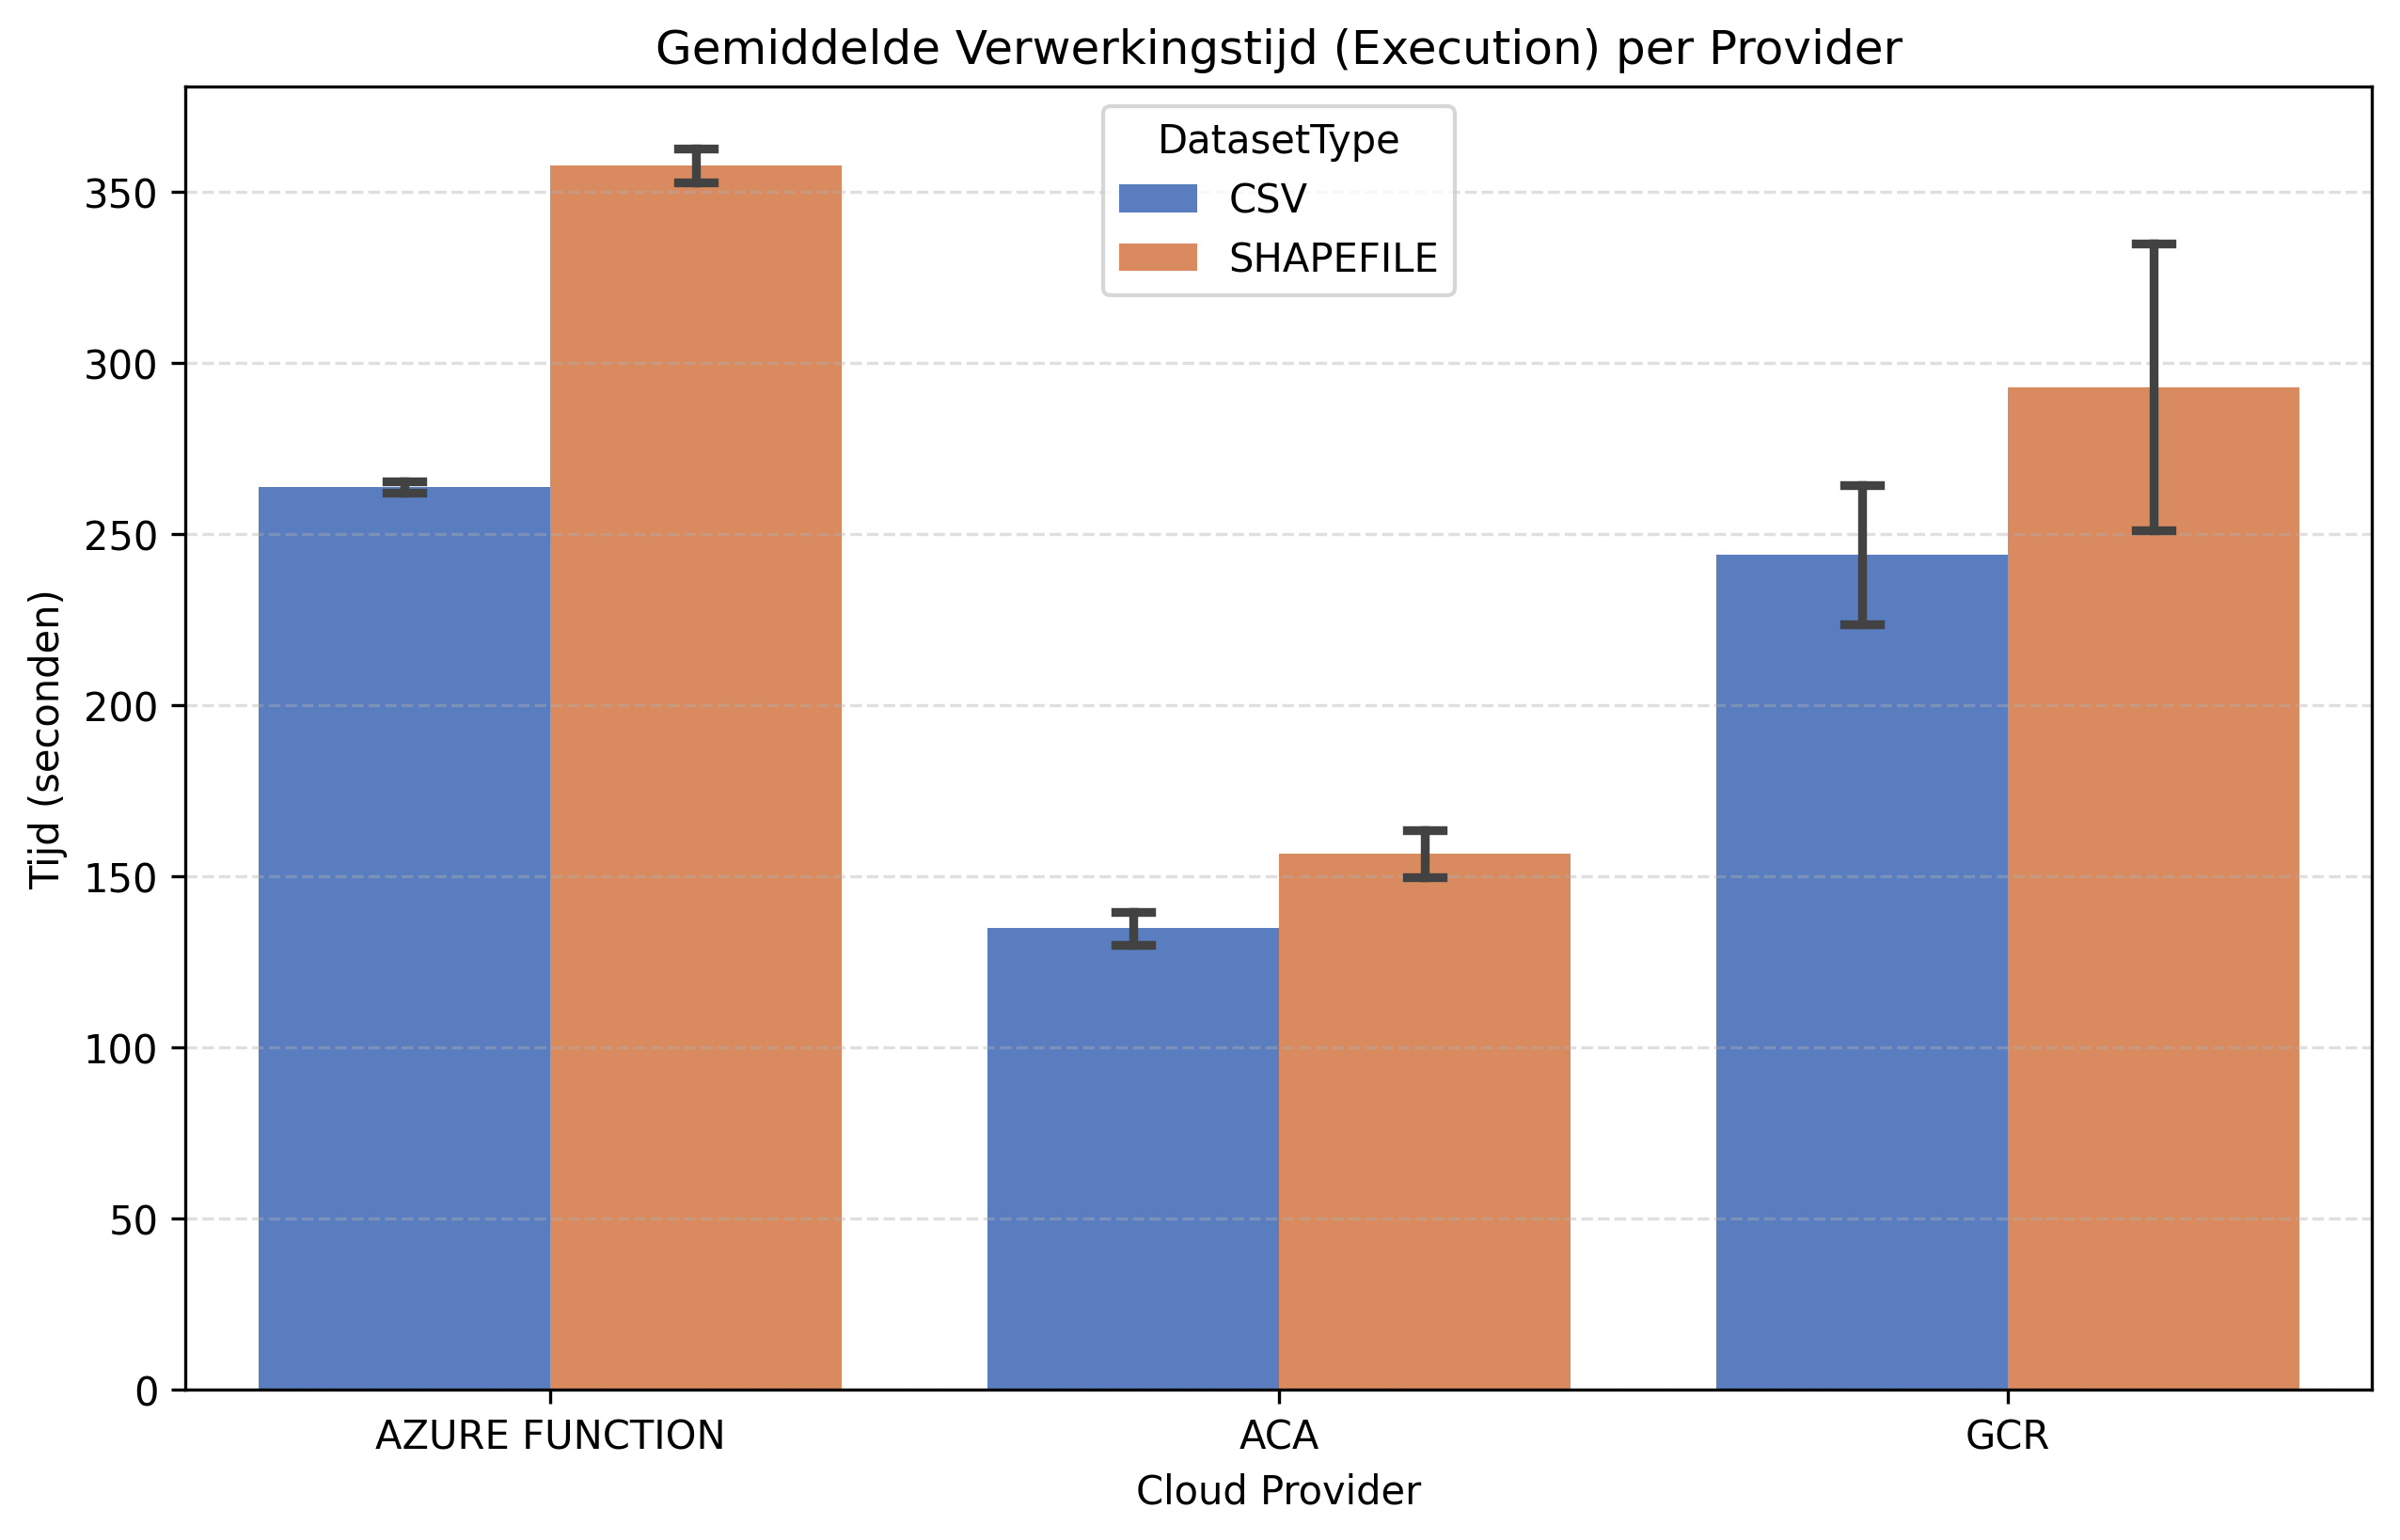
\includegraphics[width=\textwidth]{../graphics/warmstart_plotbar_verwerking.png}
    \caption{Plotbar: Gemiddelde verwerkingstijd (Execution) per provider}
\end{figure}

\begin{figure}[H]
    \centering
    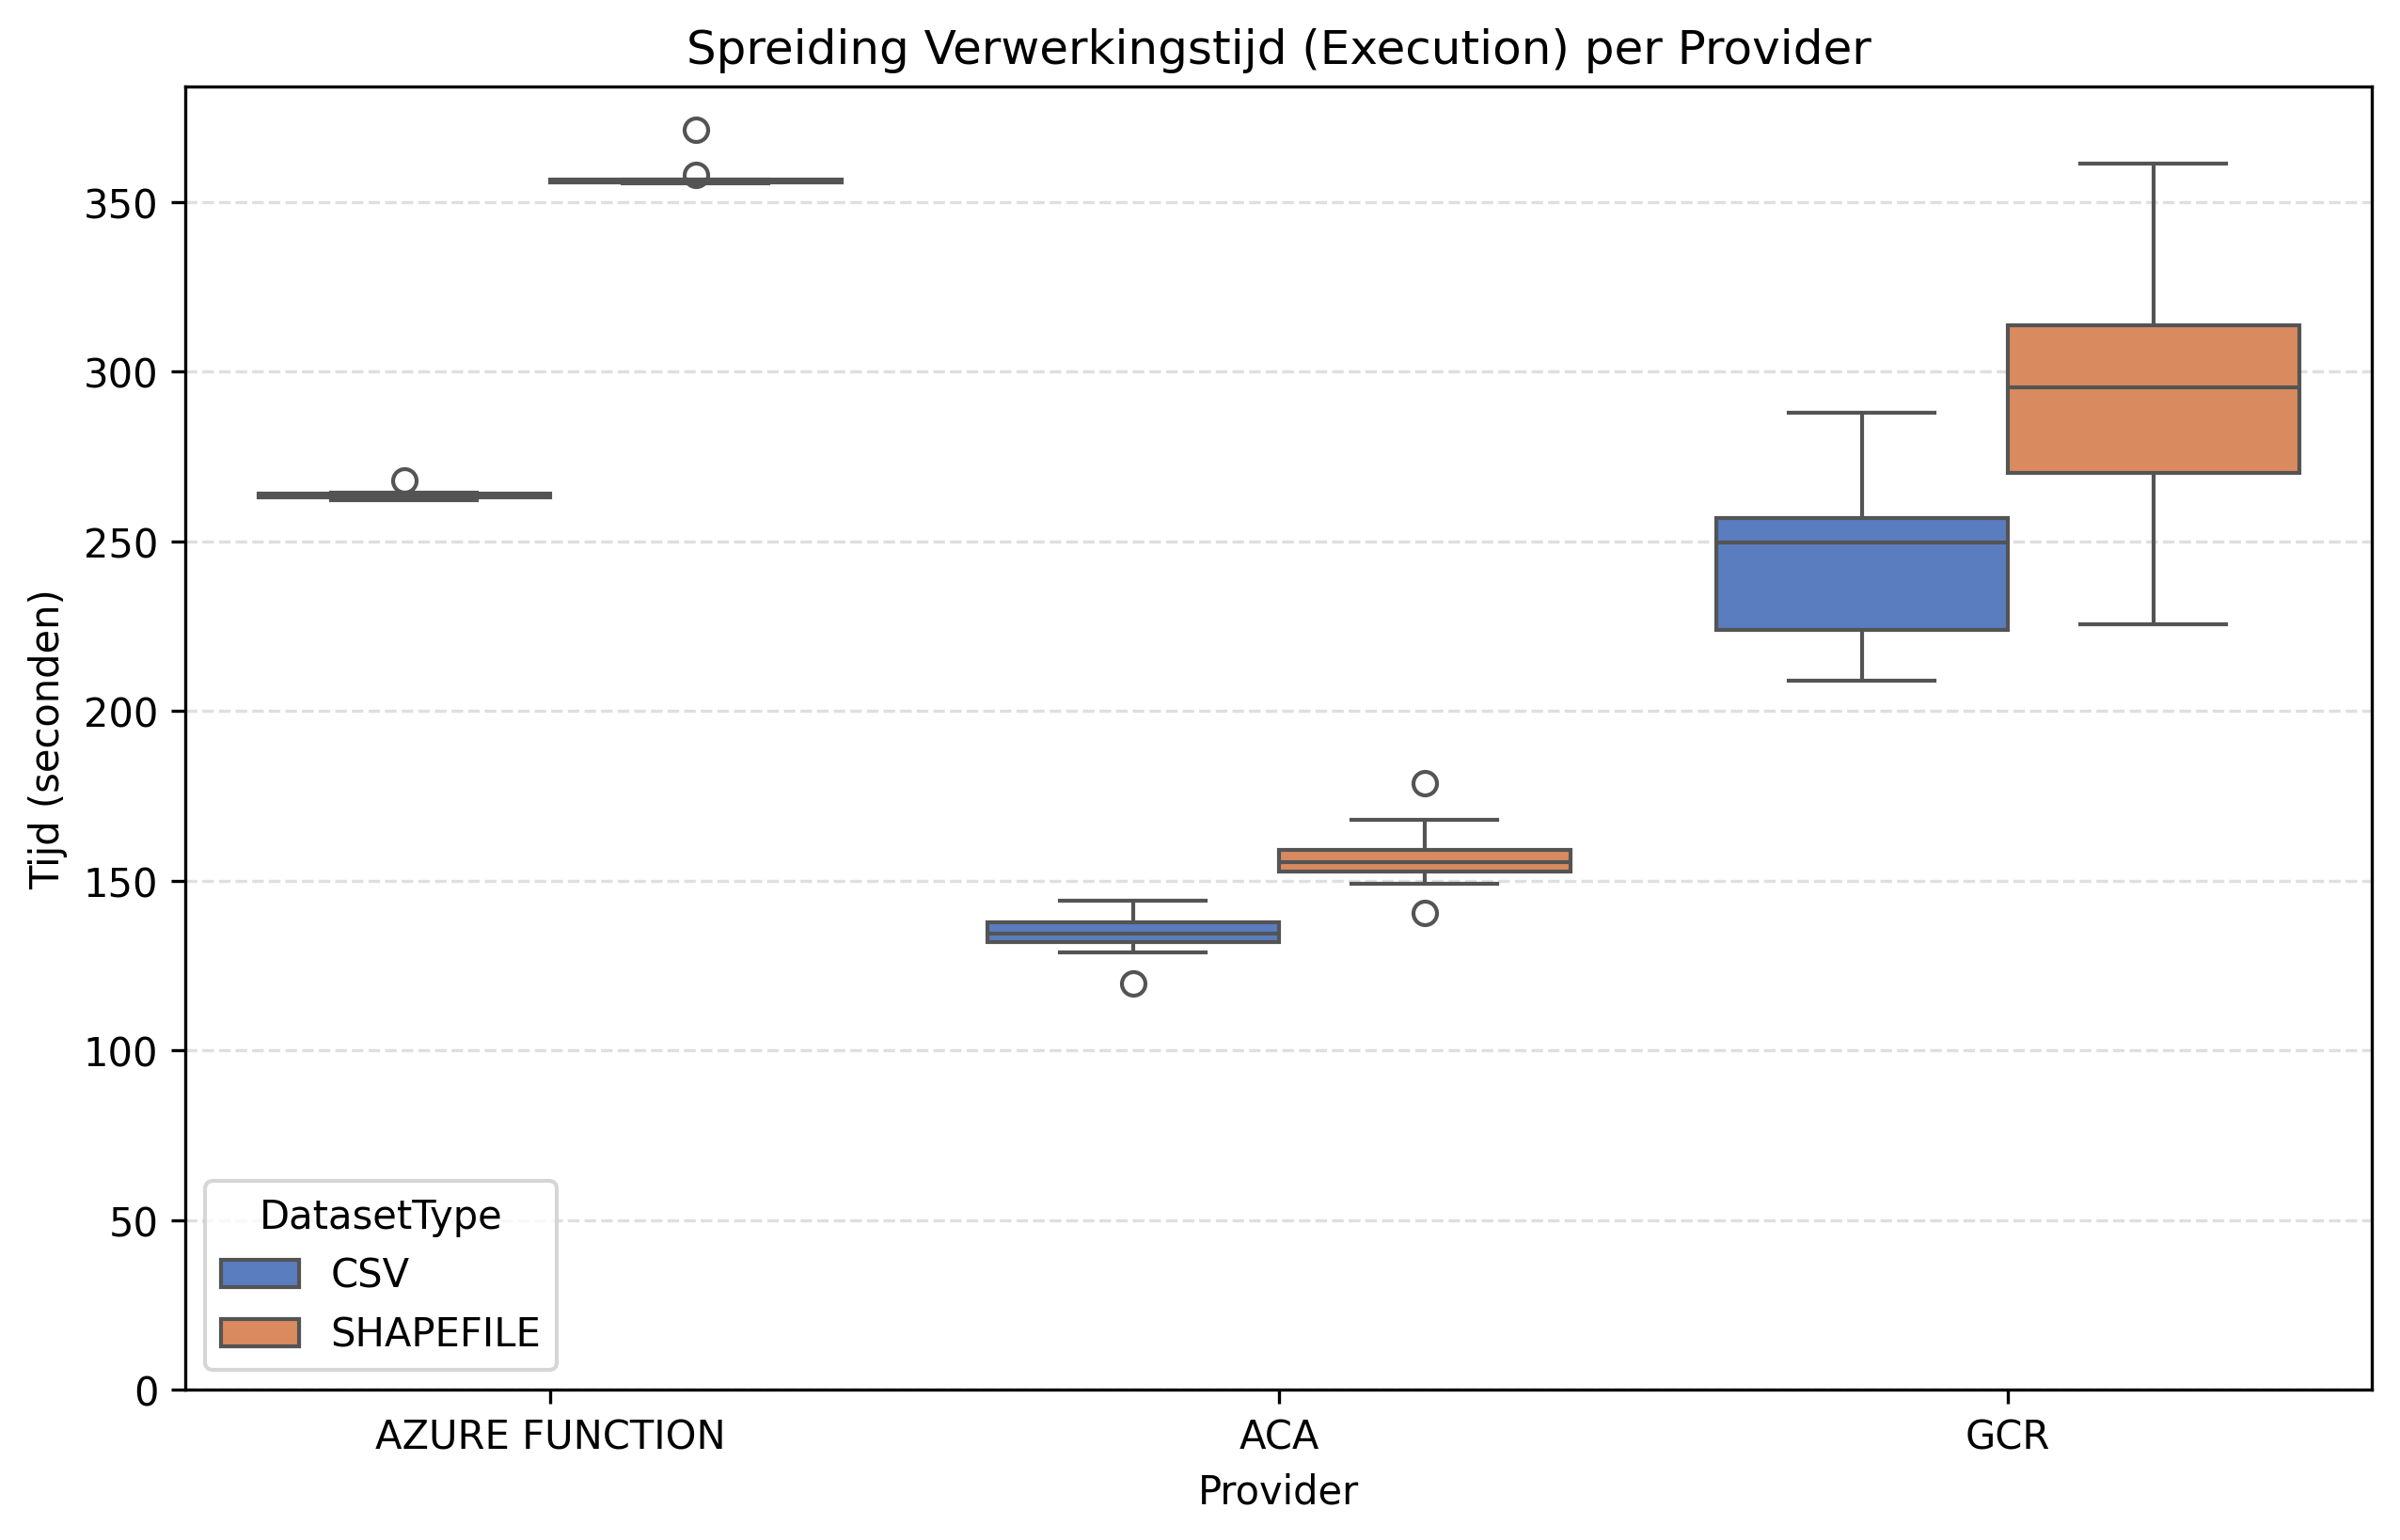
\includegraphics[width=\textwidth]{../graphics/warmstart_plotbox_verwerking.png}
    \caption{Plotbox: Spreiding verwerkingstijd (Execution) per provider}
\end{figure}

ACA is duidelijk de snelste verwerker van een dataset voor zowel CSV als voor Shapefile bij een warme start. GCR is gemiddeld ook sneller dan de huidige toepassing, maar heeft wel de meest gespreide verwerkingen geregistreerd. Dit maakt het onvoorstelbaarder dan de andere omgevingen.

\subsubsection{Hypothese H3}

\begin{description}
    \item[Stelling:] De overstap naar containers levert geen significante snelheidswinst op bij de verwerking van CSV.
    \item[Resultaat:] Verworpen ($p < 0,001$)
\end{description}

GCR (243,95s) en ACA (134,80s) zijn gemiddeld sneller met het verwerken van datasets dan de huidige functie (263,76s). Tussen de nieuwe cloud-omgevingen is er ook een duidelijke winnaar. ACA heeft bijna een snelheidswinst van 50\% ten opzichte van de Azure Function.

\subsubsection{Hypothese H4}

\begin{description}
    \item[Stelling:] GCR en ACA presteren identiek bij het genereren van complexe Shapefiles.
    \item[Resultaat:] Verworpen ($p < 0,001$)
\end{description}

De data toont duidelijk dat Shapefiles zwaarder te verwerken zijn dan CSV-bestanden. Uit deze data komt ook voort dat ACA (156,58s) ten opzichte van GCR (292,92s) het meest efficiënt is in het verwerken van deze gegevens. Bijgevolg kunnen we concluderen dat ACA superieur is in deze context.

\subsection{Totale Doorlooptijd}

\begin{figure}[H]
    \centering
    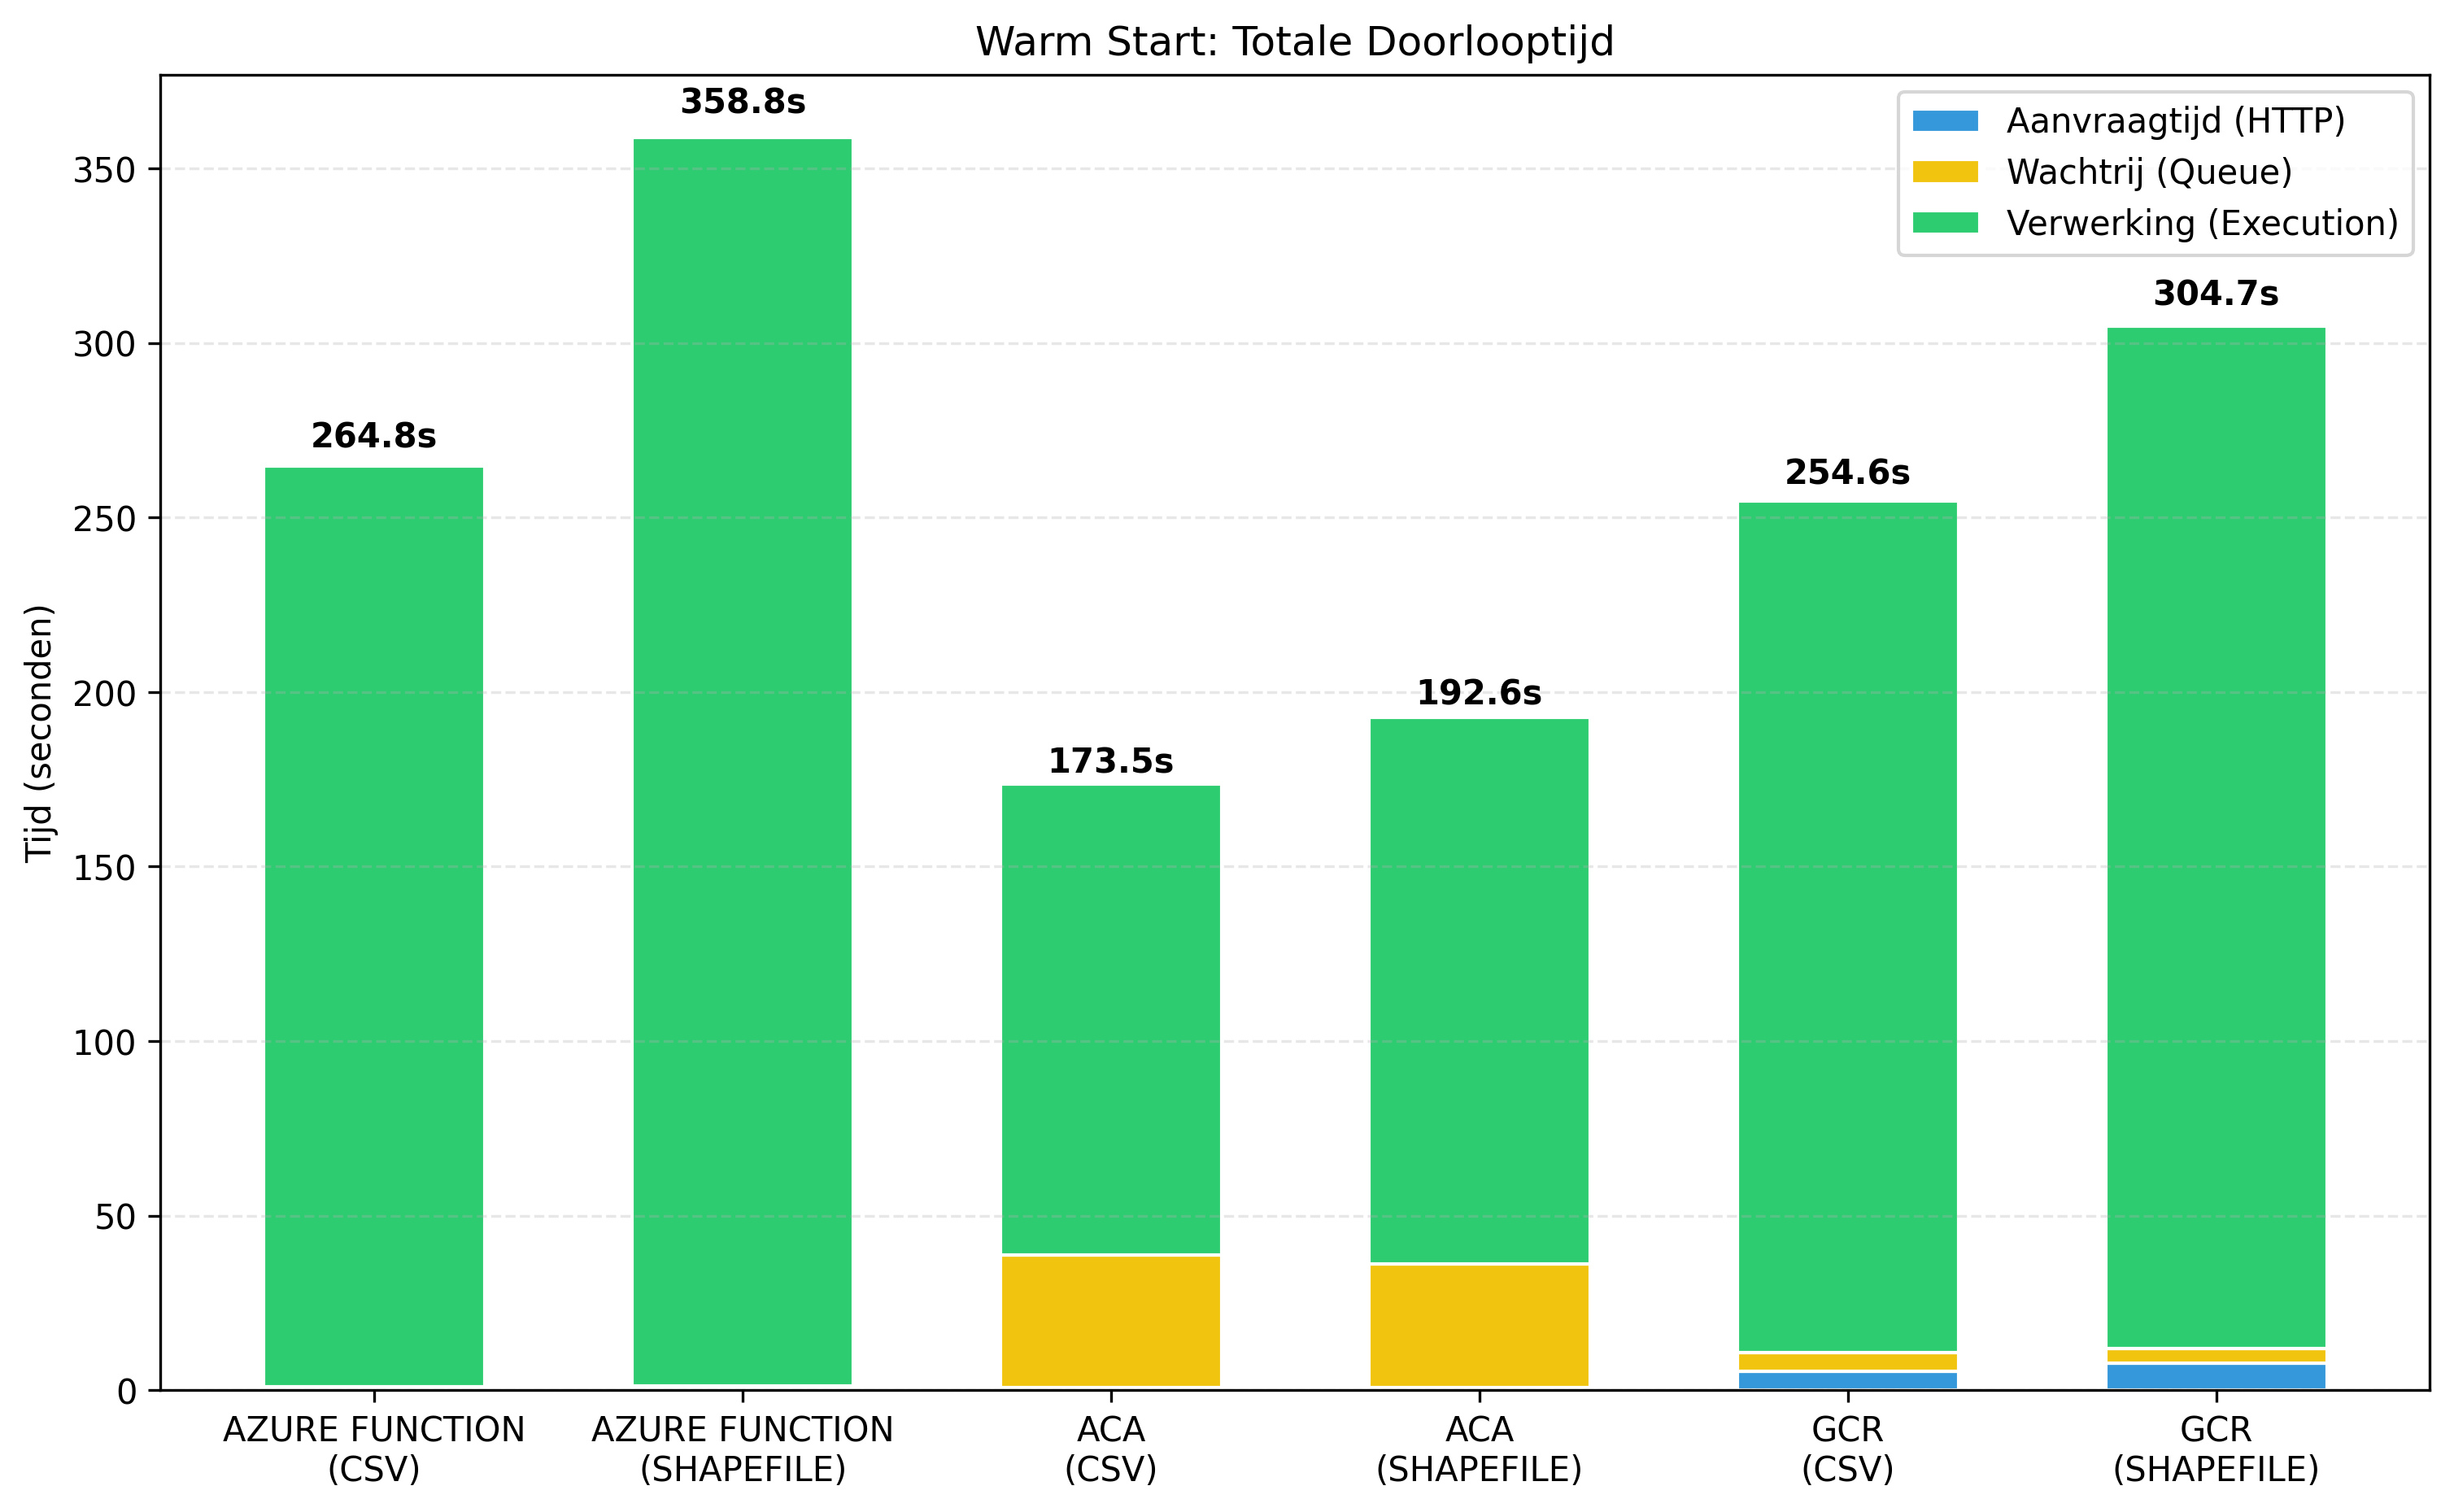
\includegraphics[width=\textwidth]{../graphics/warmstart_stacked_total.png}
    \caption{Warm start: Totale doorlooptijd}
\end{figure}

Ondanks de minder efficiënte wachtrijverwerking is ACA over het algemeen de snelste dataset-verwerker bij een warme start. GCR heeft meer overhead van het netwerk, maar is gemiddeld nog iets sneller dan de huidige toepassing. Op vlak van Shapefiles is het meer efficiënt dan bij CSV ten opzichte van de Azure Function.

\section{Cold Start: Ongunstige Omstandigheden}

Hierbij waren de containers naar 0 instanties geschaald, waardoor ze niet actief konden reageren op aanvragen.

\subsection{Aanvraagtijd}

\begin{figure}[H]
    \centering
    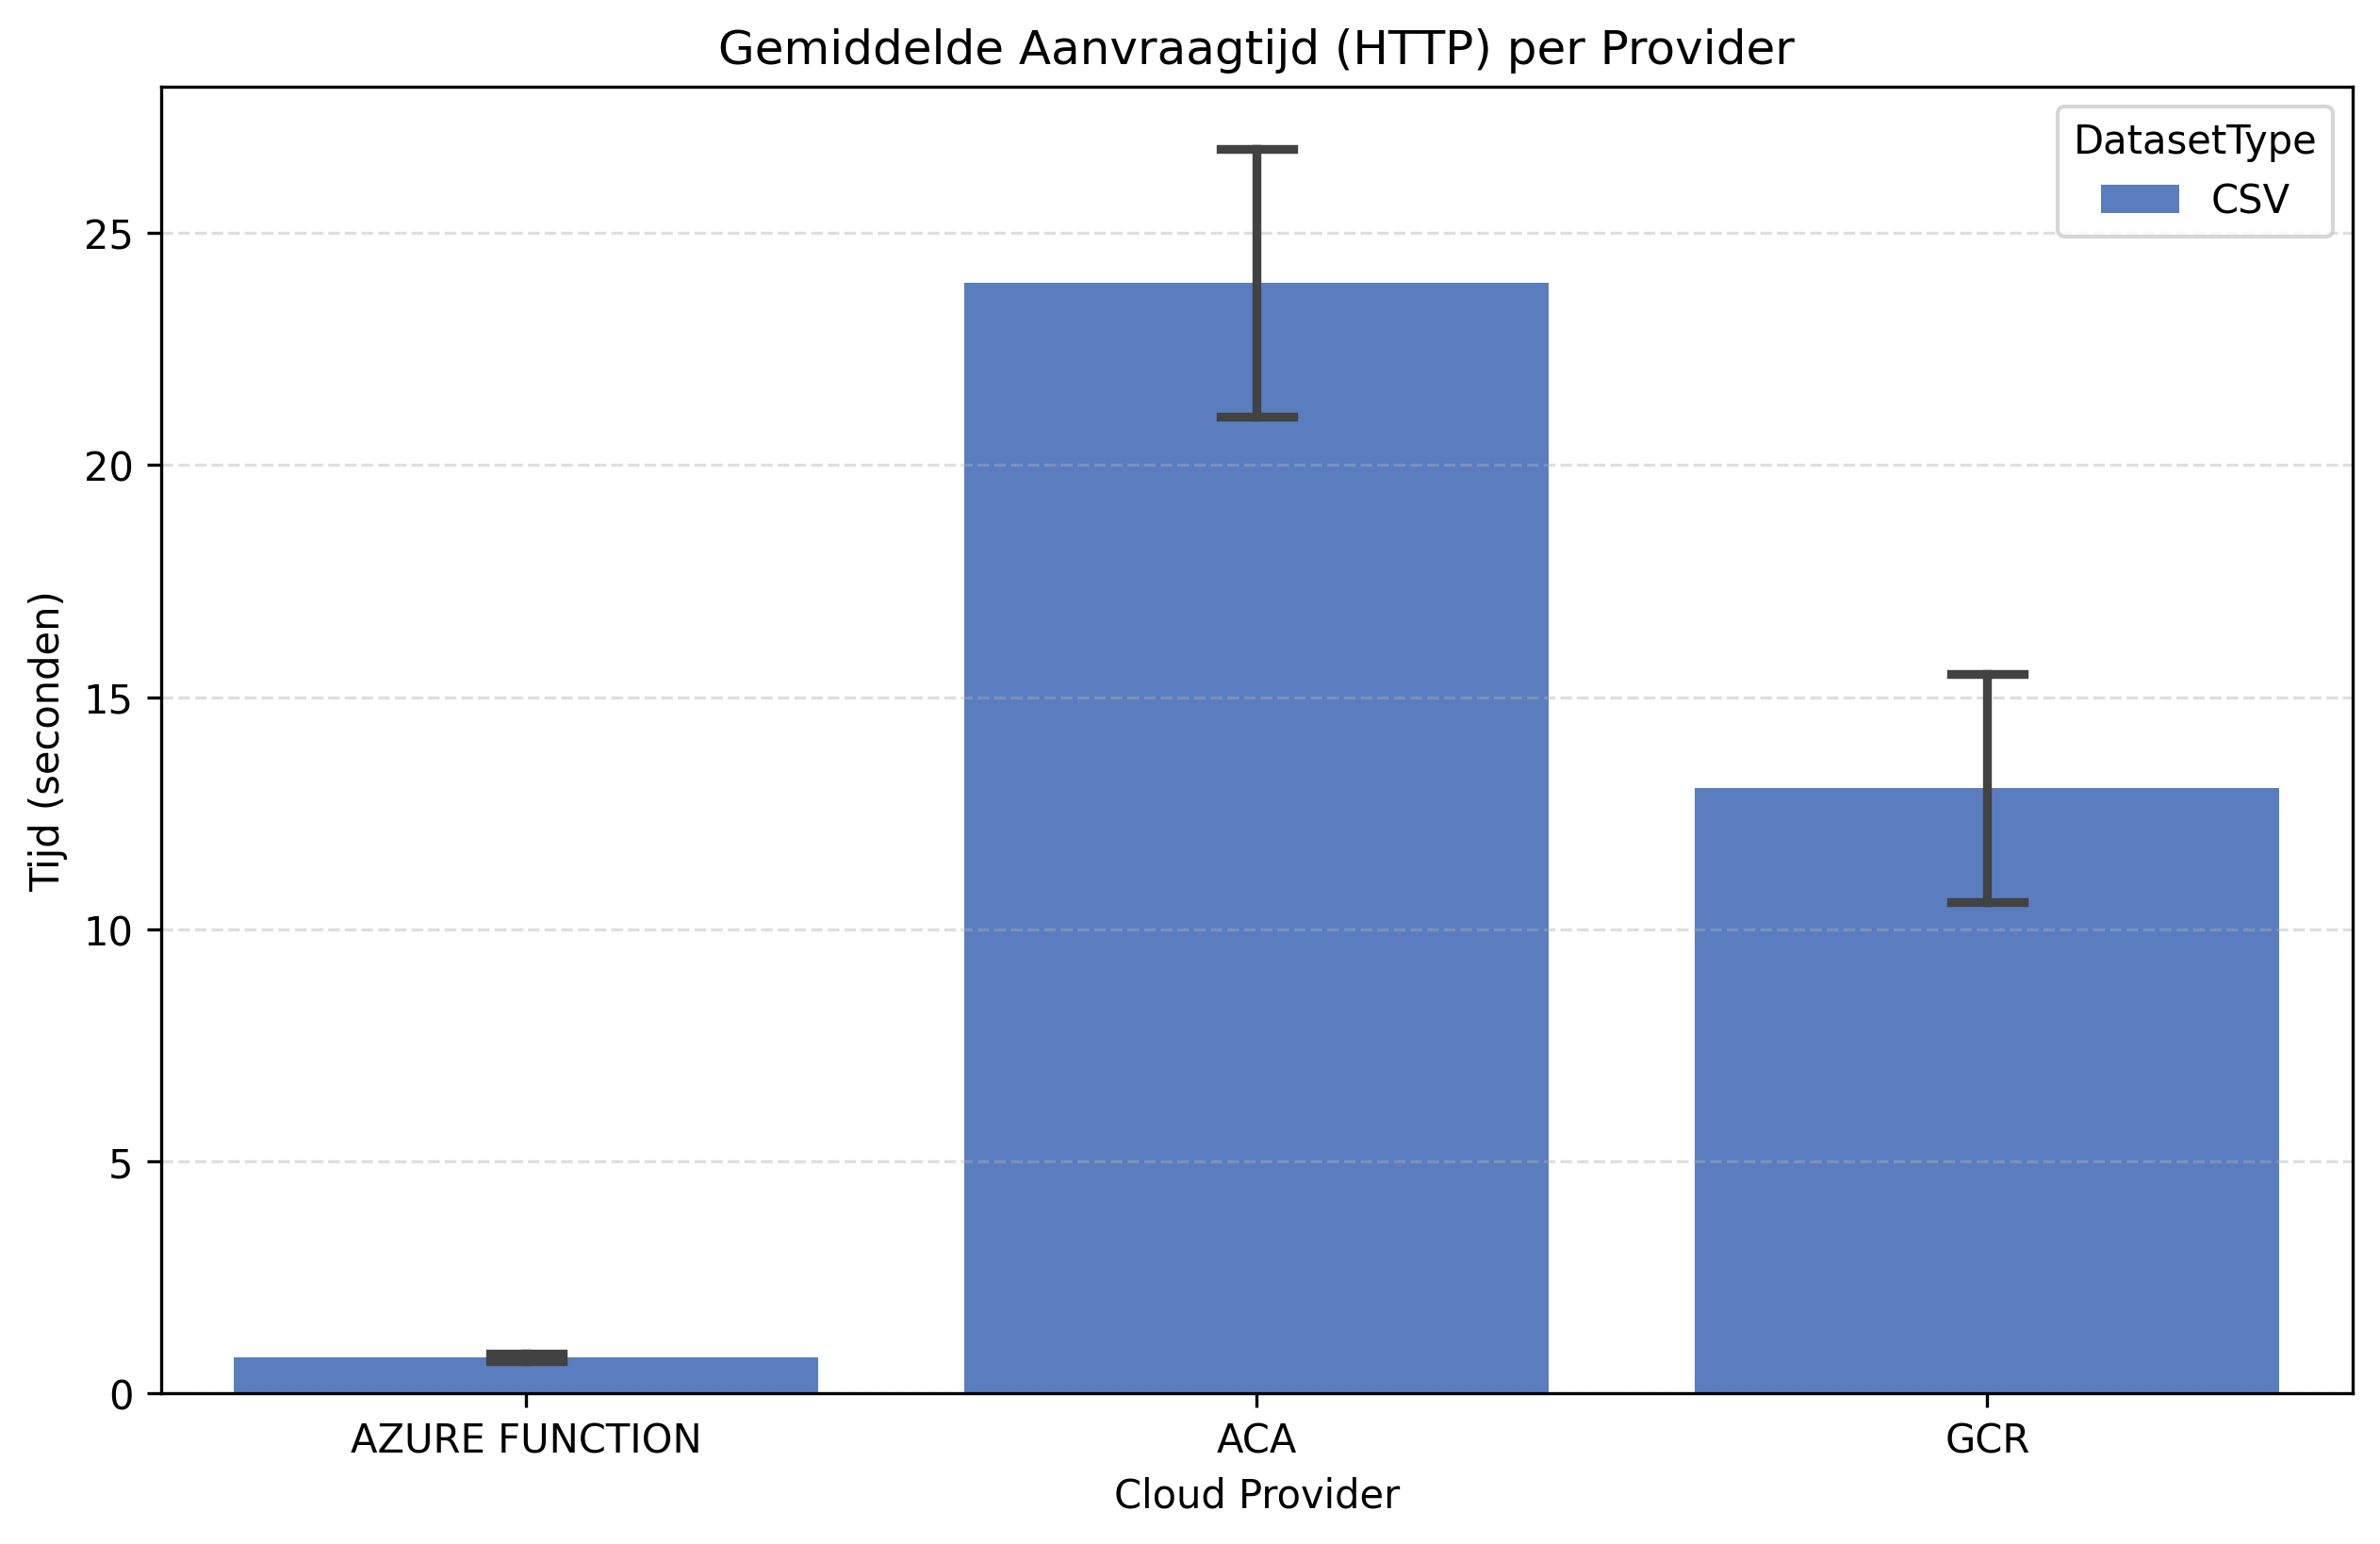
\includegraphics[width=\textwidth]{../graphics/coldstart_plotbar_http.png}
    \caption{Plotbar: Gemiddelde aanvraagtijd (HTTP) per provider}
\end{figure}

ACA heeft de meeste tijd nodig om een container op te schalen van 0. GCR voldoet volgens de grafiek ook niet aan de requirement van maximaal 10 seconden, maar komt wel dichter in de buurt. Zowel ACA als GCR hebben ongeveer dezelfde spreiding van gemiddelde aanvraagtijden, wat ze even consistent maken. Azure Function schaalt niet naar 0 en heeft dus geen last van cold starts.

\subsection{Wachtrijvertraging}

\begin{figure}[H]
    \centering
    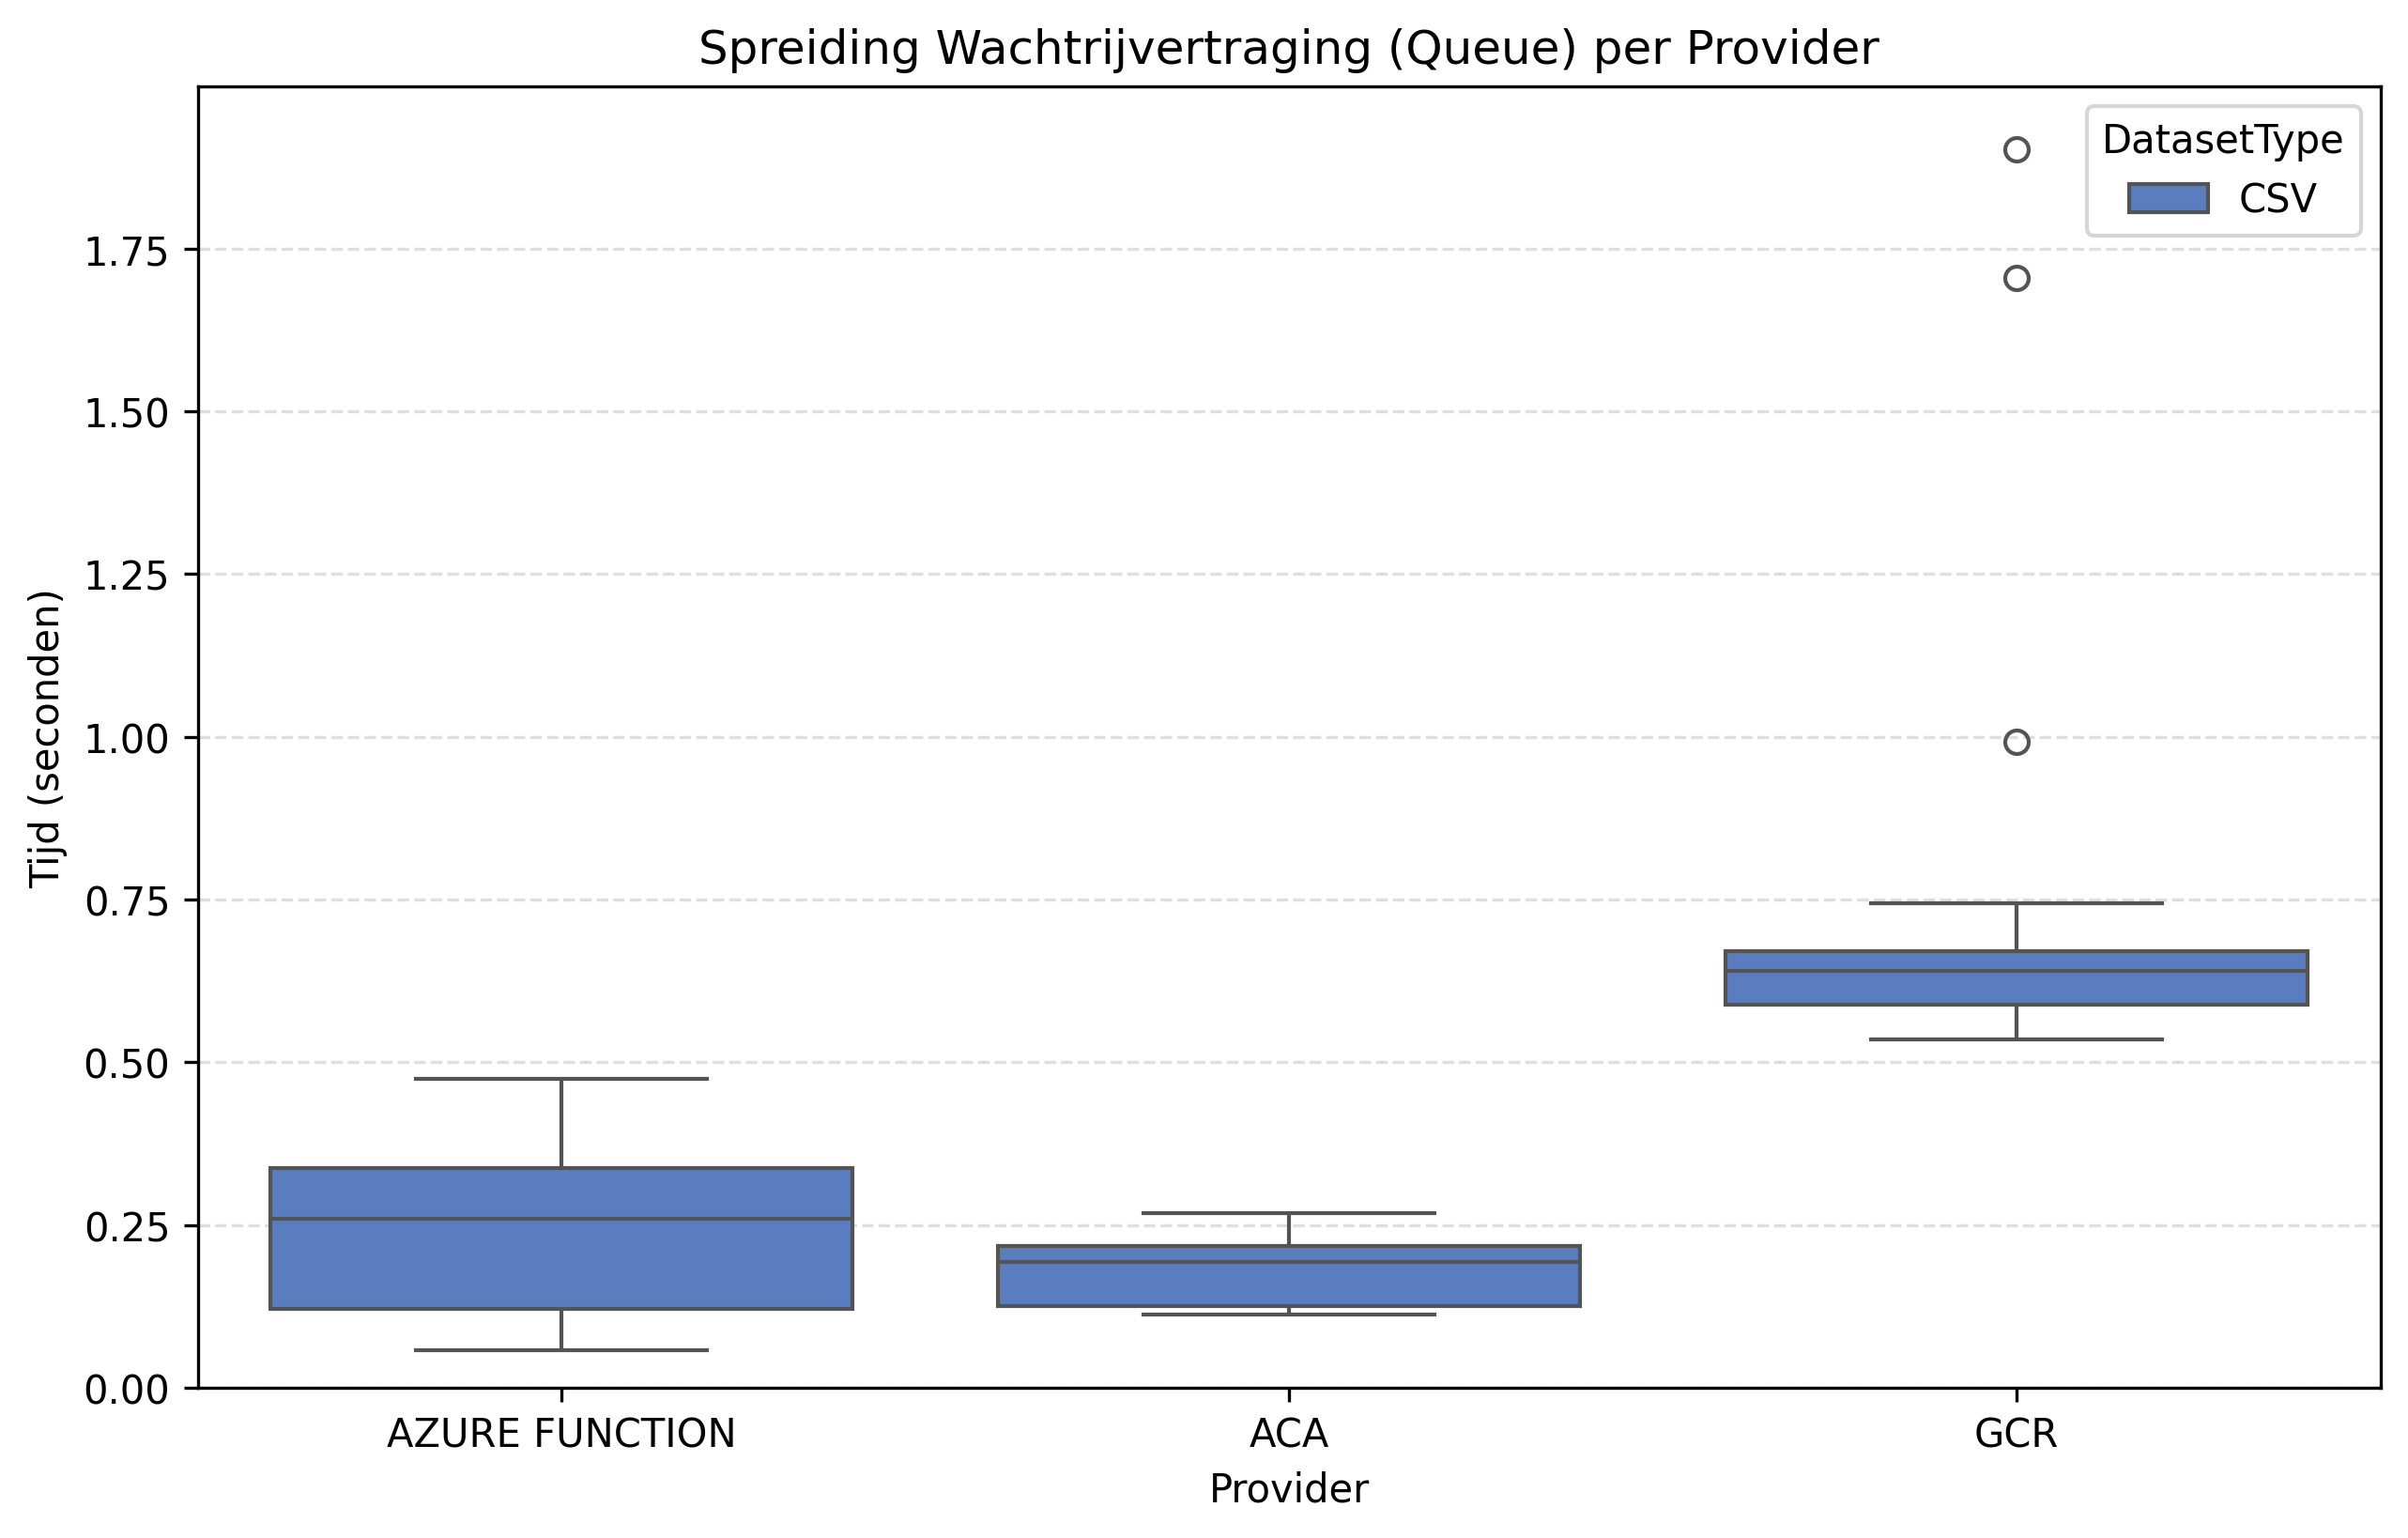
\includegraphics[width=\textwidth]{../graphics/coldstart_plotbox_queue.png}
    \caption{Plotbar: Spreiding wachtrijvertraging (Queue) per provider}
\end{figure}

Wat hier opvalt is dat ACA, ondanks de langere aanvraagtijd, wel sneller een container aan een job koppelt dan GCR. De wachtrijvertraging is ook de meest consistente van de 3. Daartegenover heeft GCR meer moeite bij dit gegeven en is dit ook te zien in de spreiding van de tijden. 

\subsection{Verwerkingstijd}

\begin{figure}[H]
    \centering
    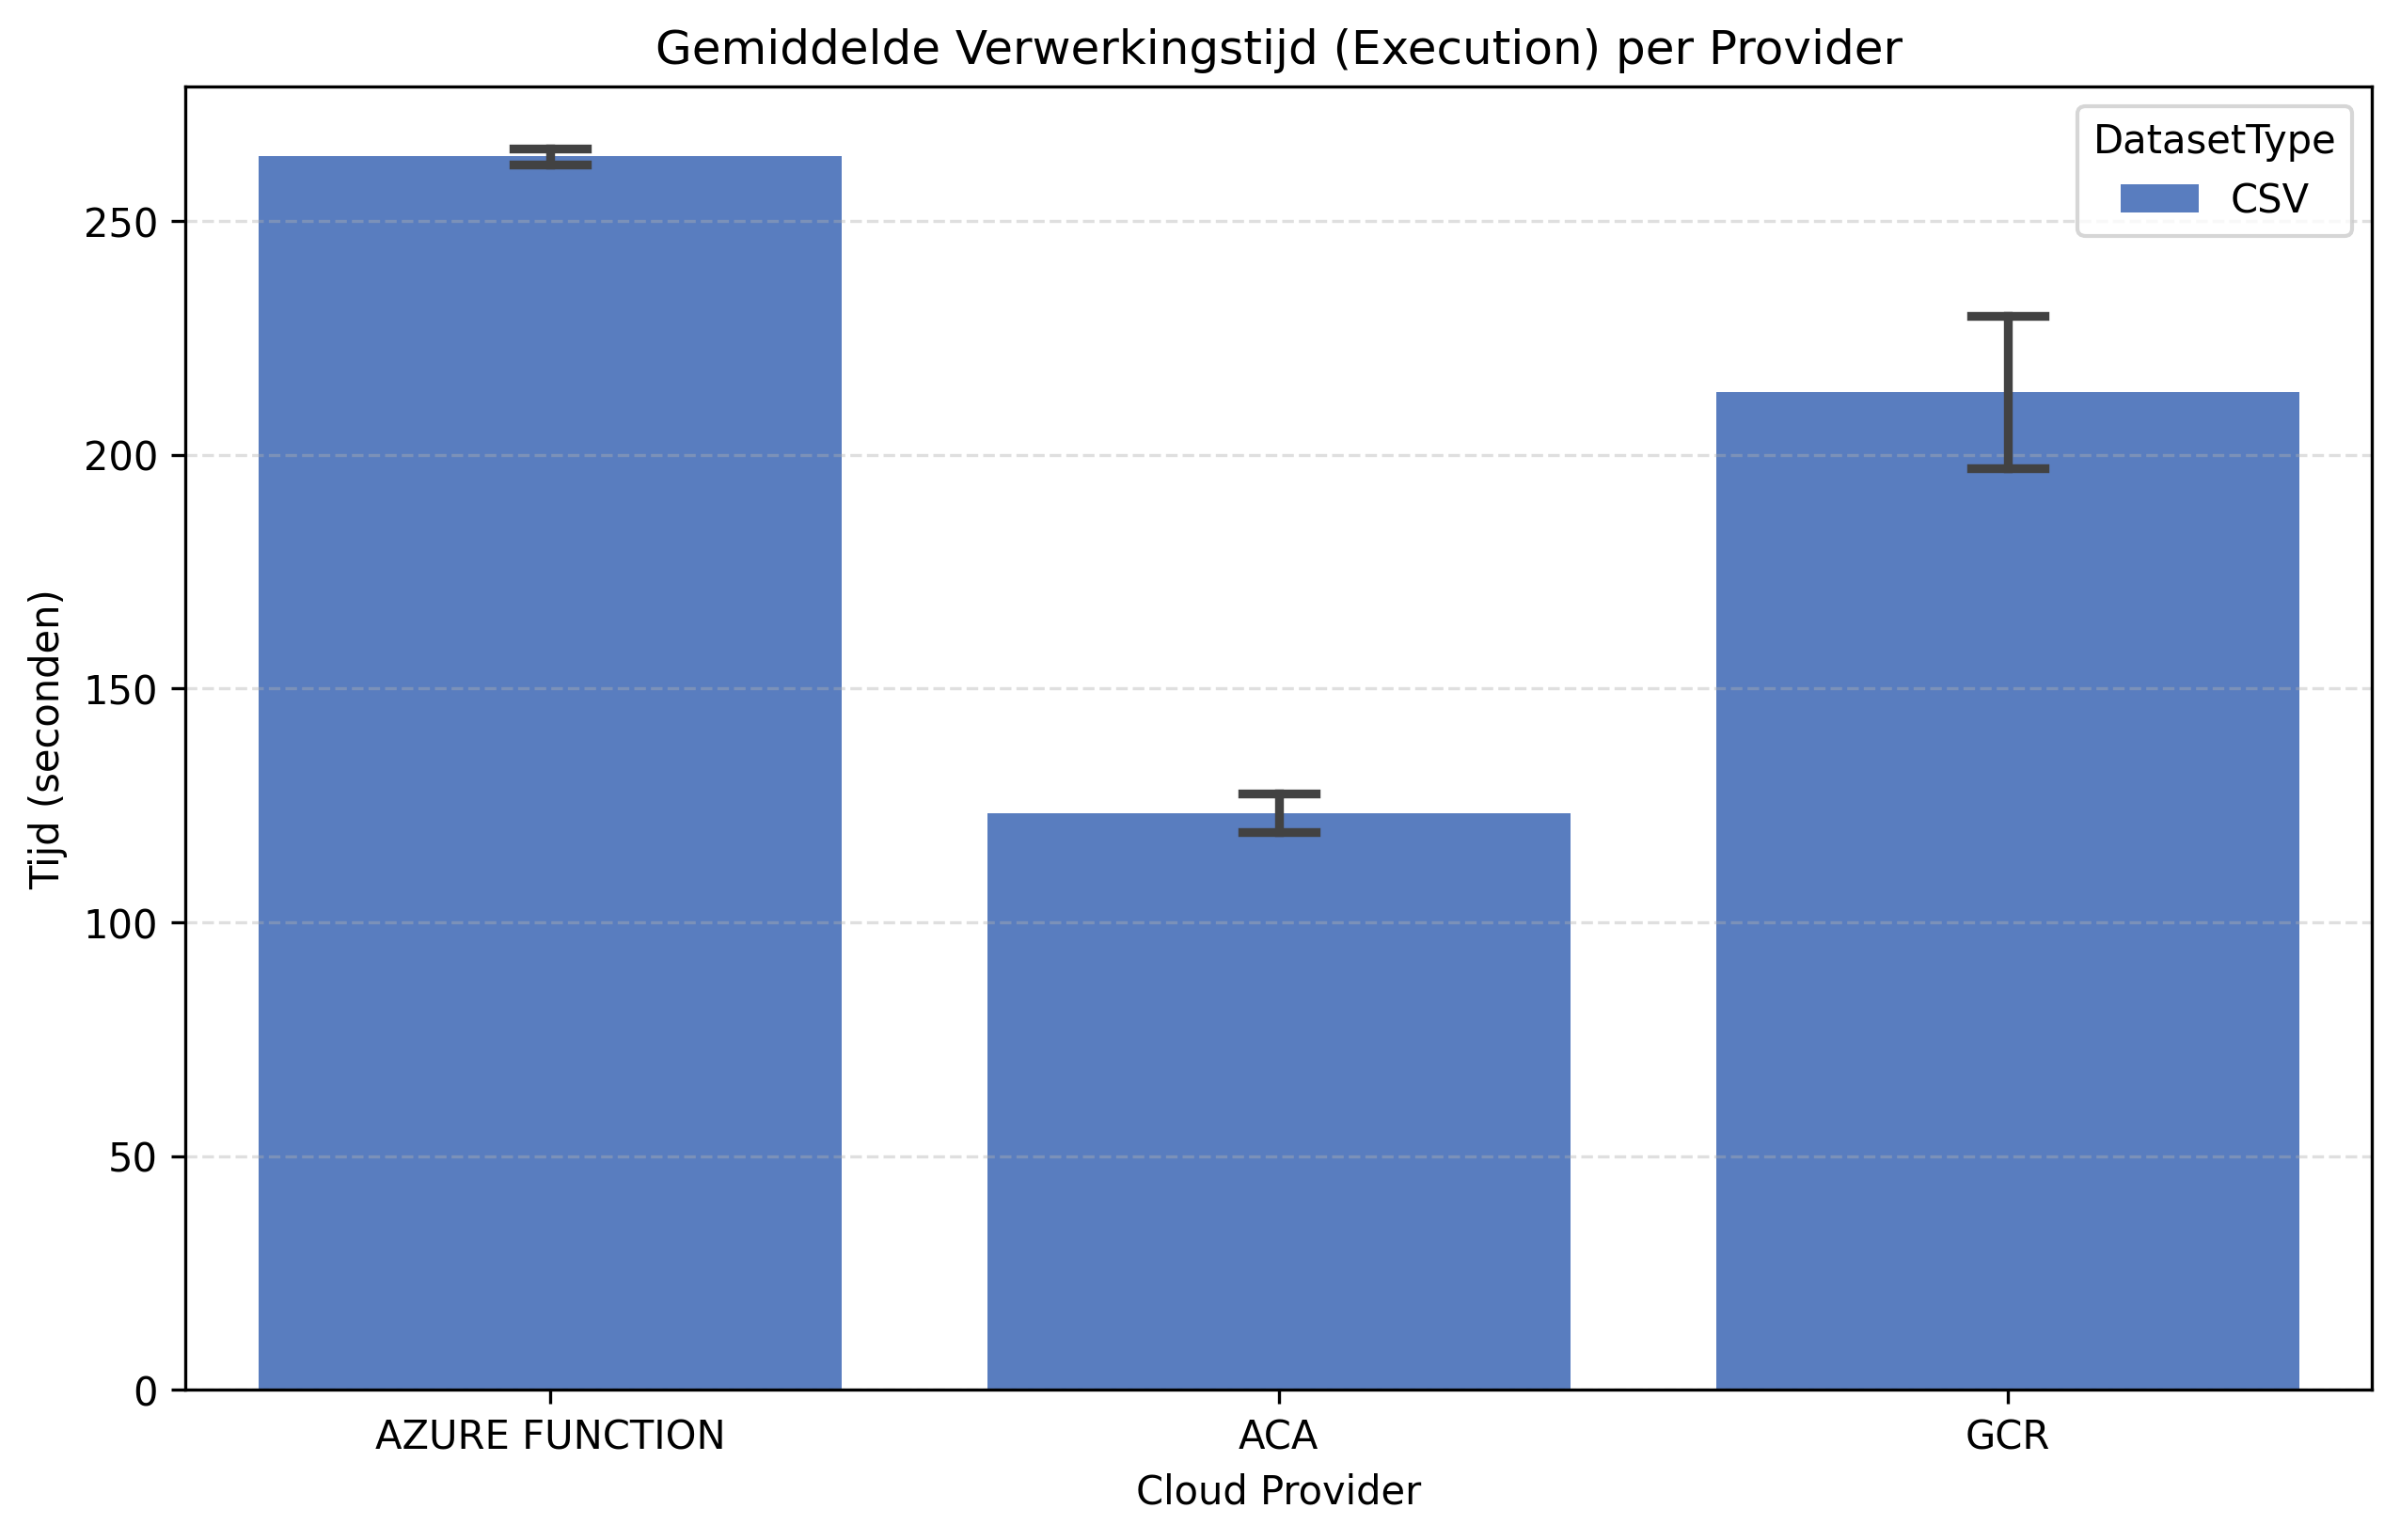
\includegraphics[width=\textwidth]{../graphics/coldstart_plotbar_verwerking.png}
    \caption{Plotbar: Gemiddelde verwerkingstijd (Execution) per provider}
\end{figure}

De meest efficiënte achtergrondverwerking is voor ACA met de meest consistente spreiding bij een cold start (Azure Function heeft geen cold start). 

\subsection{Totale Doorlooptijd}

\begin{figure}[H]
    \centering
    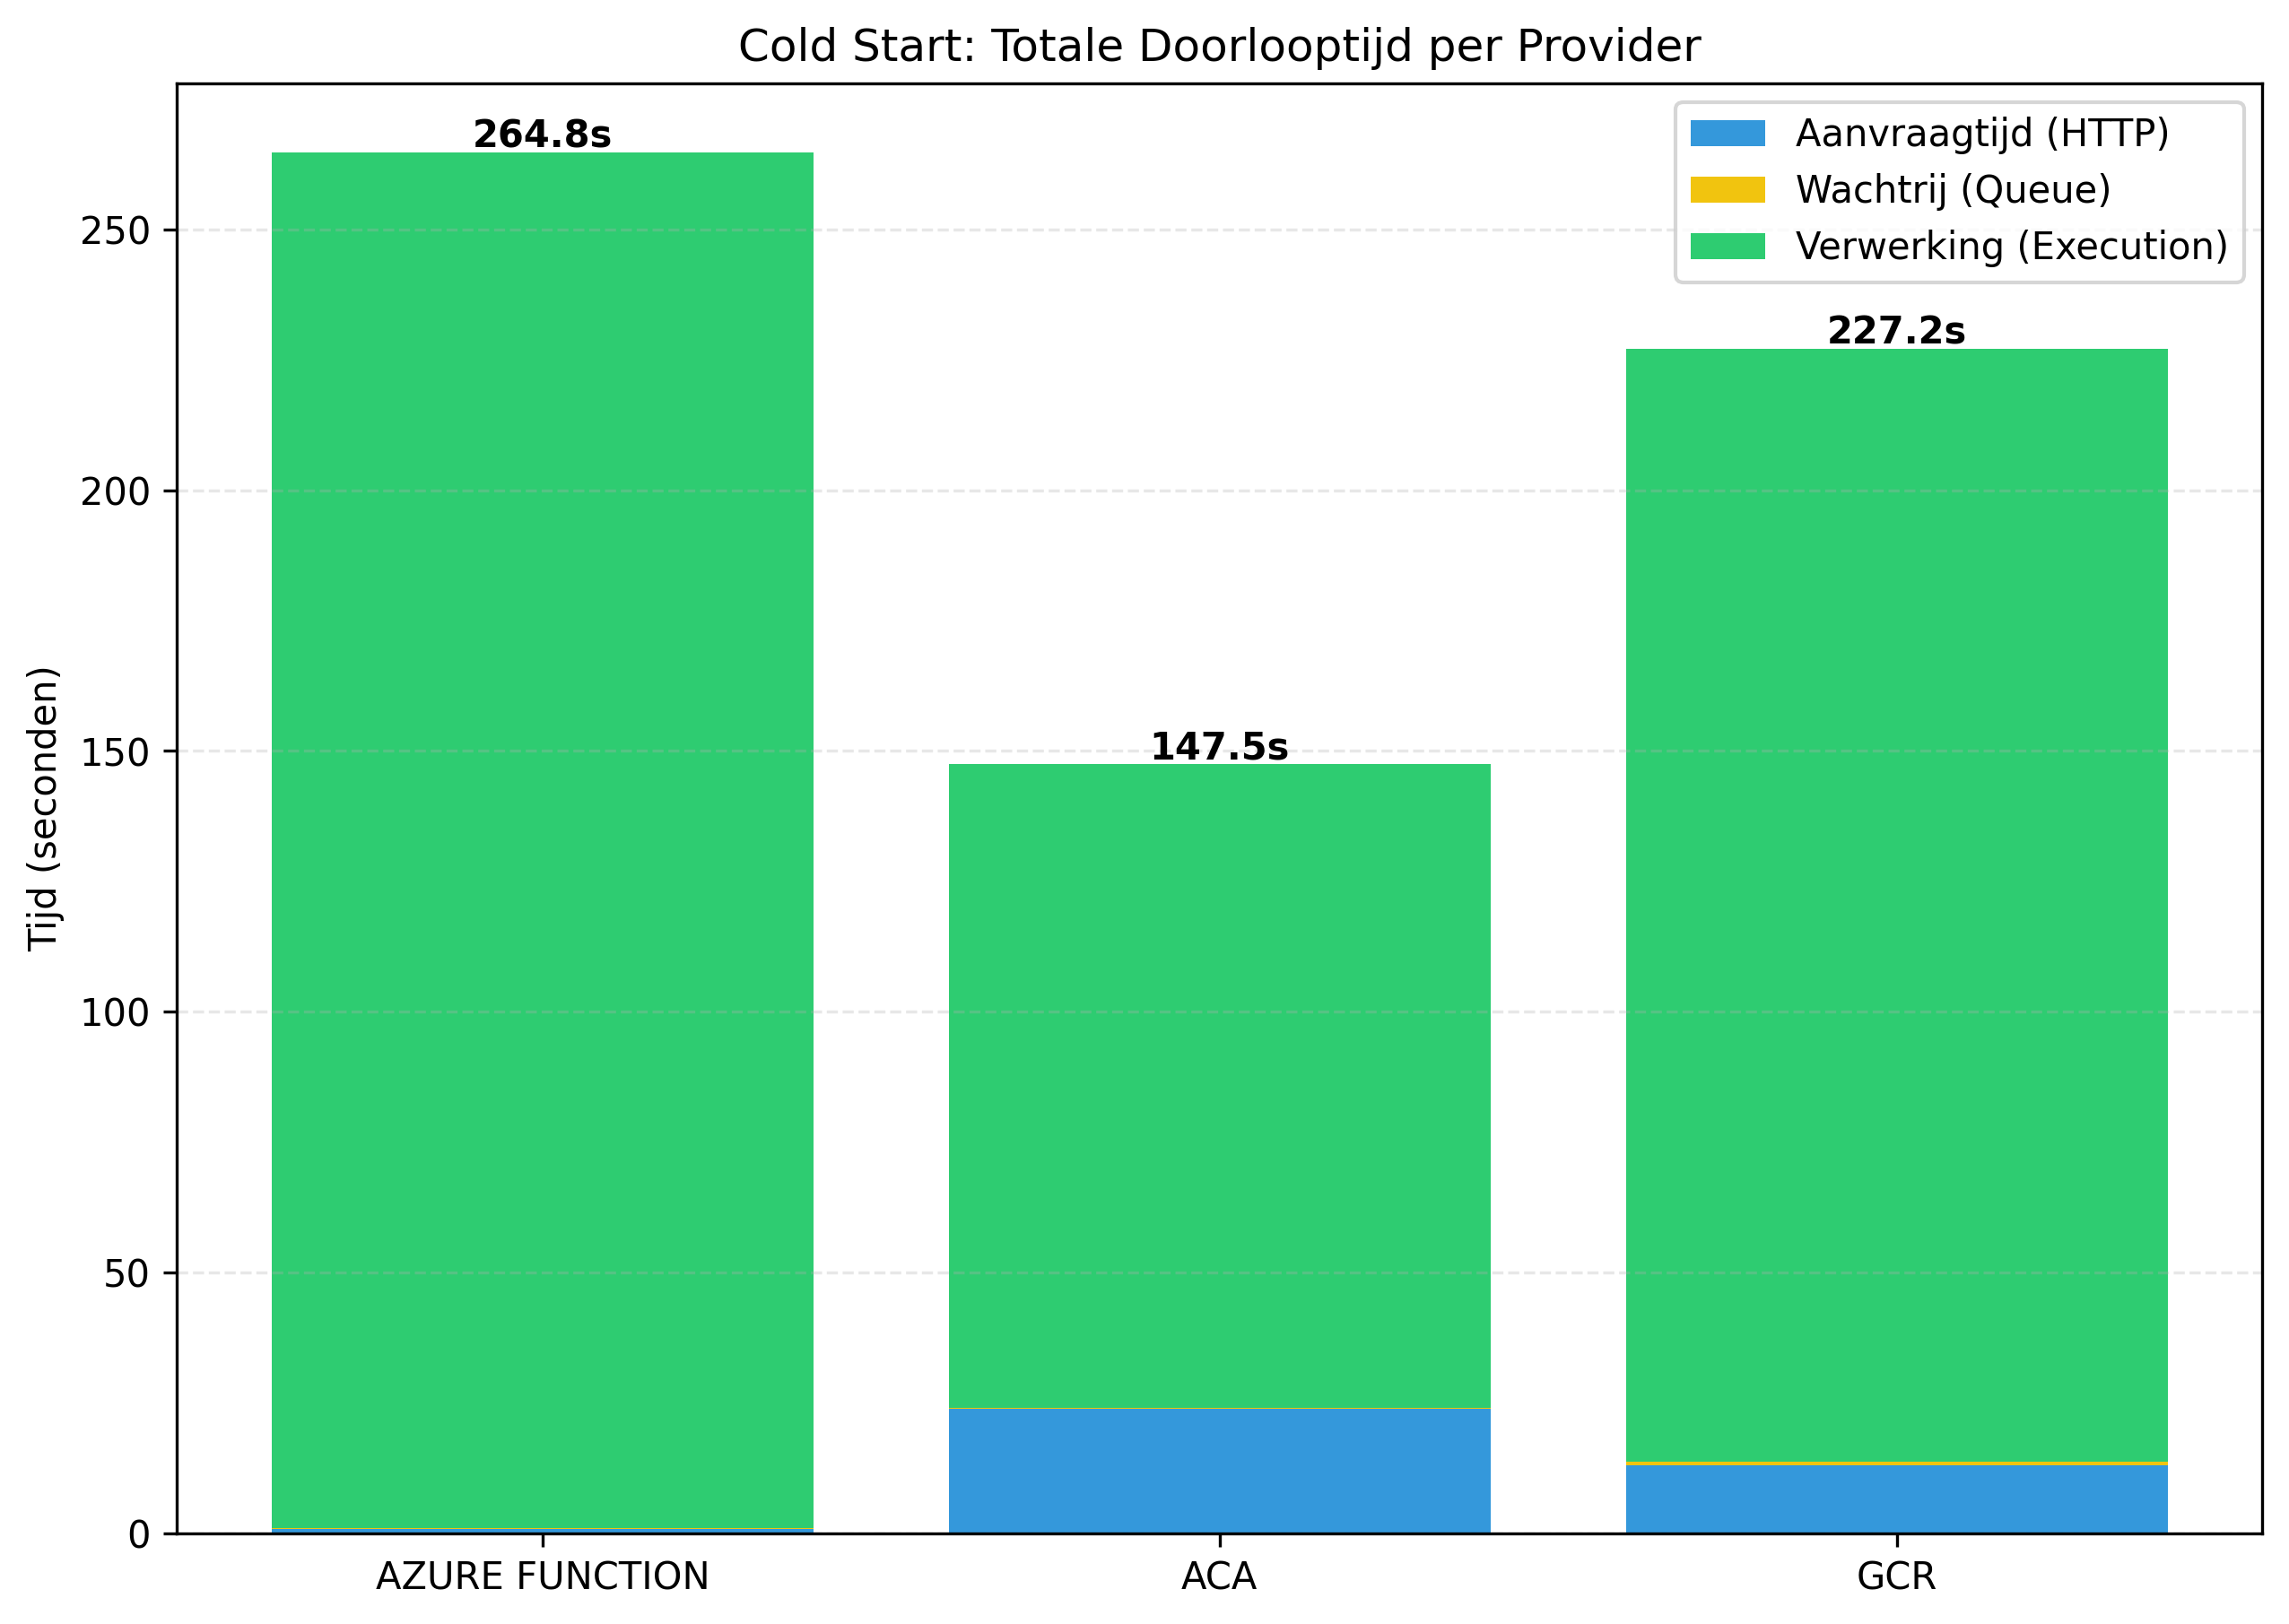
\includegraphics[width=\textwidth]{../graphics/coldstart_stacked_total.png}
    \caption{Cold start: Totale doorlooptijd}
\end{figure}

ACA is wederom de meeste efficiënte verwerker als we kijken naar de gehele doorlooptijd. Ondanks de grote overhead van de container-initialisatie, compenseert het dit door een snelle achtergrond- en wachtrijverwerking.

\subsubsection{Hypothese H5}

\begin{description}
    \item[Stelling:] De totale doorlooptijd van een ``koude'' container is niet trager dan de huidige ``warme'' Baseline.
    \item[Resultaat:] Verworpen ($p < 0,001$)
\end{description}

ACA (147,48s) en GCR (227,16s) zijn sneller dan de Azure Function (311,81s) die warm draait. De trage opstart van containers wordt ruimschoots gecompenseerd door de moderne infrastructuur.

\subsubsection{Hypothese H6}

\begin{description}
    \item[Stelling:] Er is geen statistisch verschil in de cold start-vertraging tussen Google Cloud en Azure Container Apps.
    \item[Resultaat:] Verworpen ($p < 0,001$)
\end{description}

Beide omgevingen ondervinden een vertraging door container-initialisatie. Deze is bij ACA groter dan bij GCR, maar wordt volledig gecompenseerd bij de totale doorlooptijd door een efficiënte verwerking.

\section{Elasticiteit: Schaalbaarheid onder de Loep}

Om te testen hoe de nieuwe cloud-omgevingen reageren op piekbelasting, werd er een stresstest uitgevoerd. Deze test gaat aantonen of de omgevingen stabiel reageren en of deze betrouwbaar de berichten afhandelen onder druk.

\subsection{Stabiliteit}

\begin{figure}[H]
    \centering
    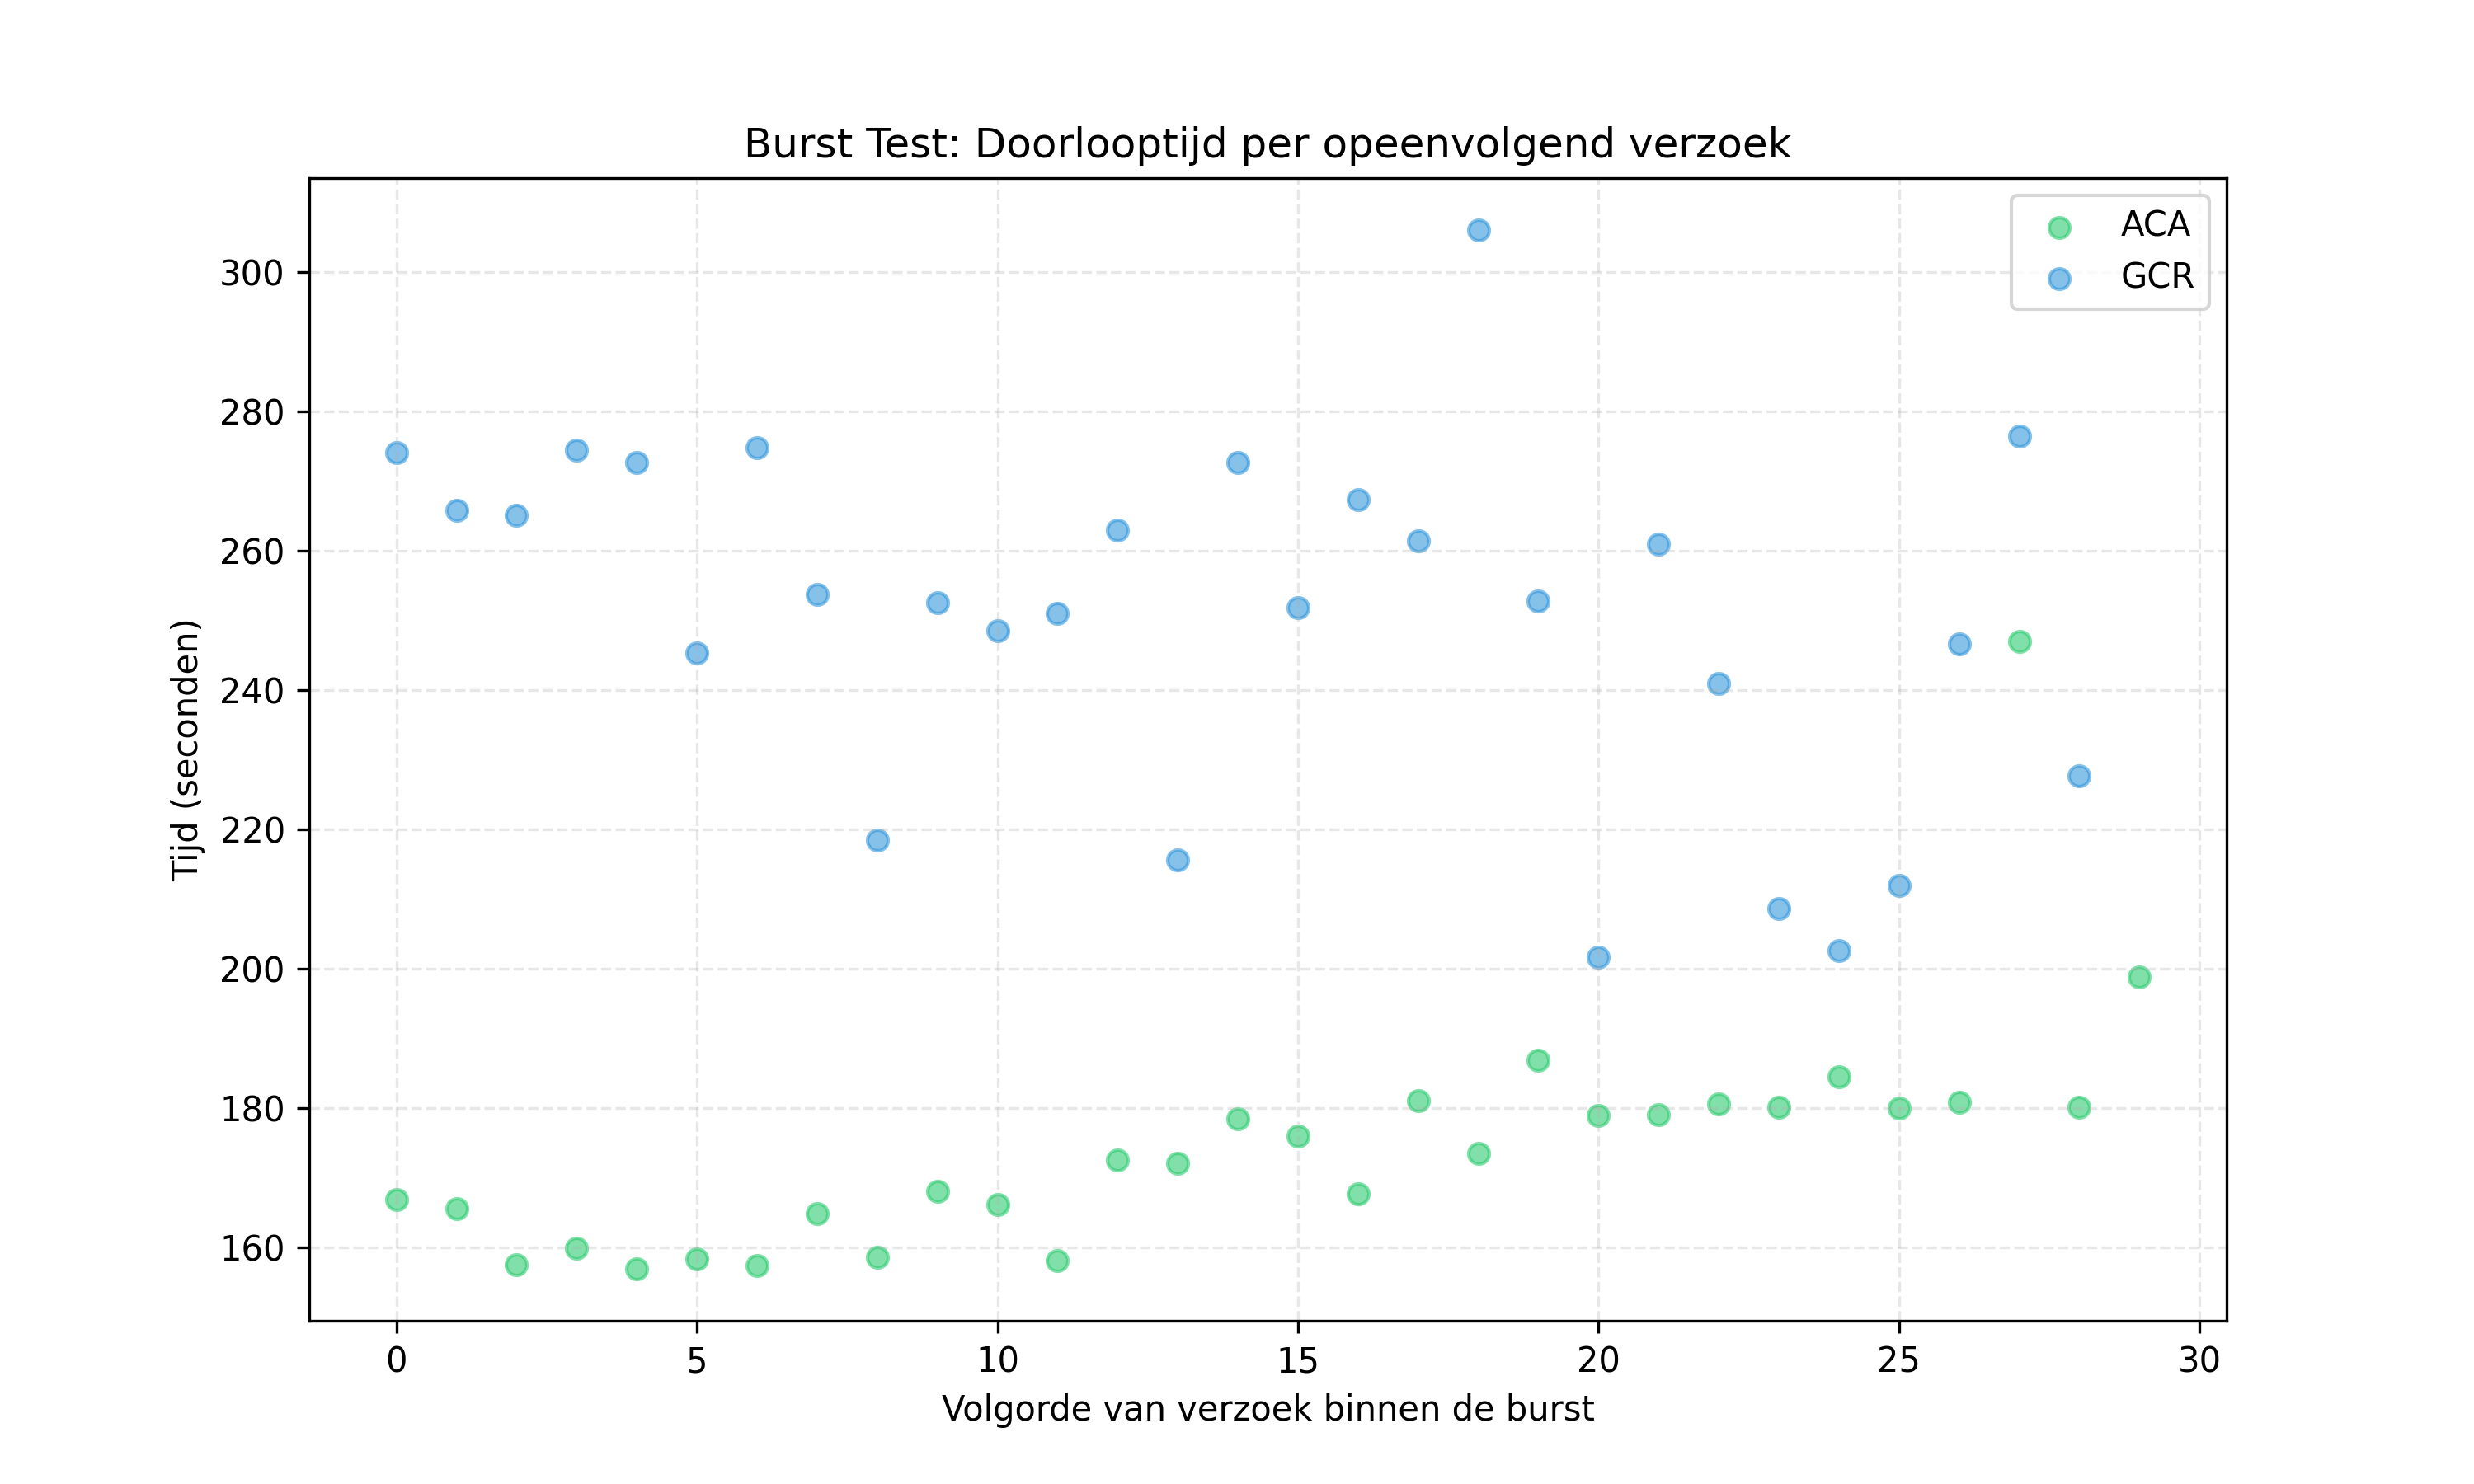
\includegraphics[width=\textwidth]{../graphics/burst_scatter_stabiliteit.png}
    \caption{Burst: Doorlooptijd per opeenvolgend verzoek}
\end{figure}

In de grafiek lijkt ACA naarmate de burst test het einde nadert meer moeite te krijgen met de verwerking en organisatie van de berichten. Wat ook opvalt, is dat ACA ondanks de toenemende druk nog steeds de meest efficiënte doorlooptijd heeft. GCR lijkt een meer stabiele verwerking te hebben, maar de spreiding van deze afhandelingen liggen wel verder uit elkaar.

\subsubsection{Hypothese H7}

\begin{description}
    \item[Stelling:] De orchestrator van GCR en ACA reageren even snel op gelijktijdige verzoeken.
    \item[Resultaat:] Verworpen ($p < 0,001$)
\end{description}

Bij GCR (3,66s) blijft de orchestrator heel stabiel. Bij ACA (36,90s) daarentegen lijkt dit steeds meer moeite te hebben met het bijbenen van de berichten en lijkt de orchestrator te bezwijken onder de druk. Google Cloud Run is dus veel beter in het verwerken van grote hoeveelheden gelijktijdige aanvragen.

\subsubsection{Hypothese H8} %TODO: naar Totale doorlooptijd?

\begin{description}
    \item[Stelling:] De doorlooptijd is onafhankelijk van de volgorde van het verzoek.
    \item[Resultaat:] Verworpen ($p < 0,001$)
\end{description}

Bij ACA is er sprake van \textit{congestie} en wordt dit in de statistische toets aangetoond door een Rho van 0,88. Verzoeken die later in de wachtrij komen, moeten steeds langer wachten om verwerkt te worden. Bij GCR is er een Rho van -0,42 die aangeeft dat de verwerking stabiel blijft of zelfs efficiënter wordt naarmate de burst vordert.

\subsection{Betrouwbaarheid}

\begin{figure}[H]
    \centering
    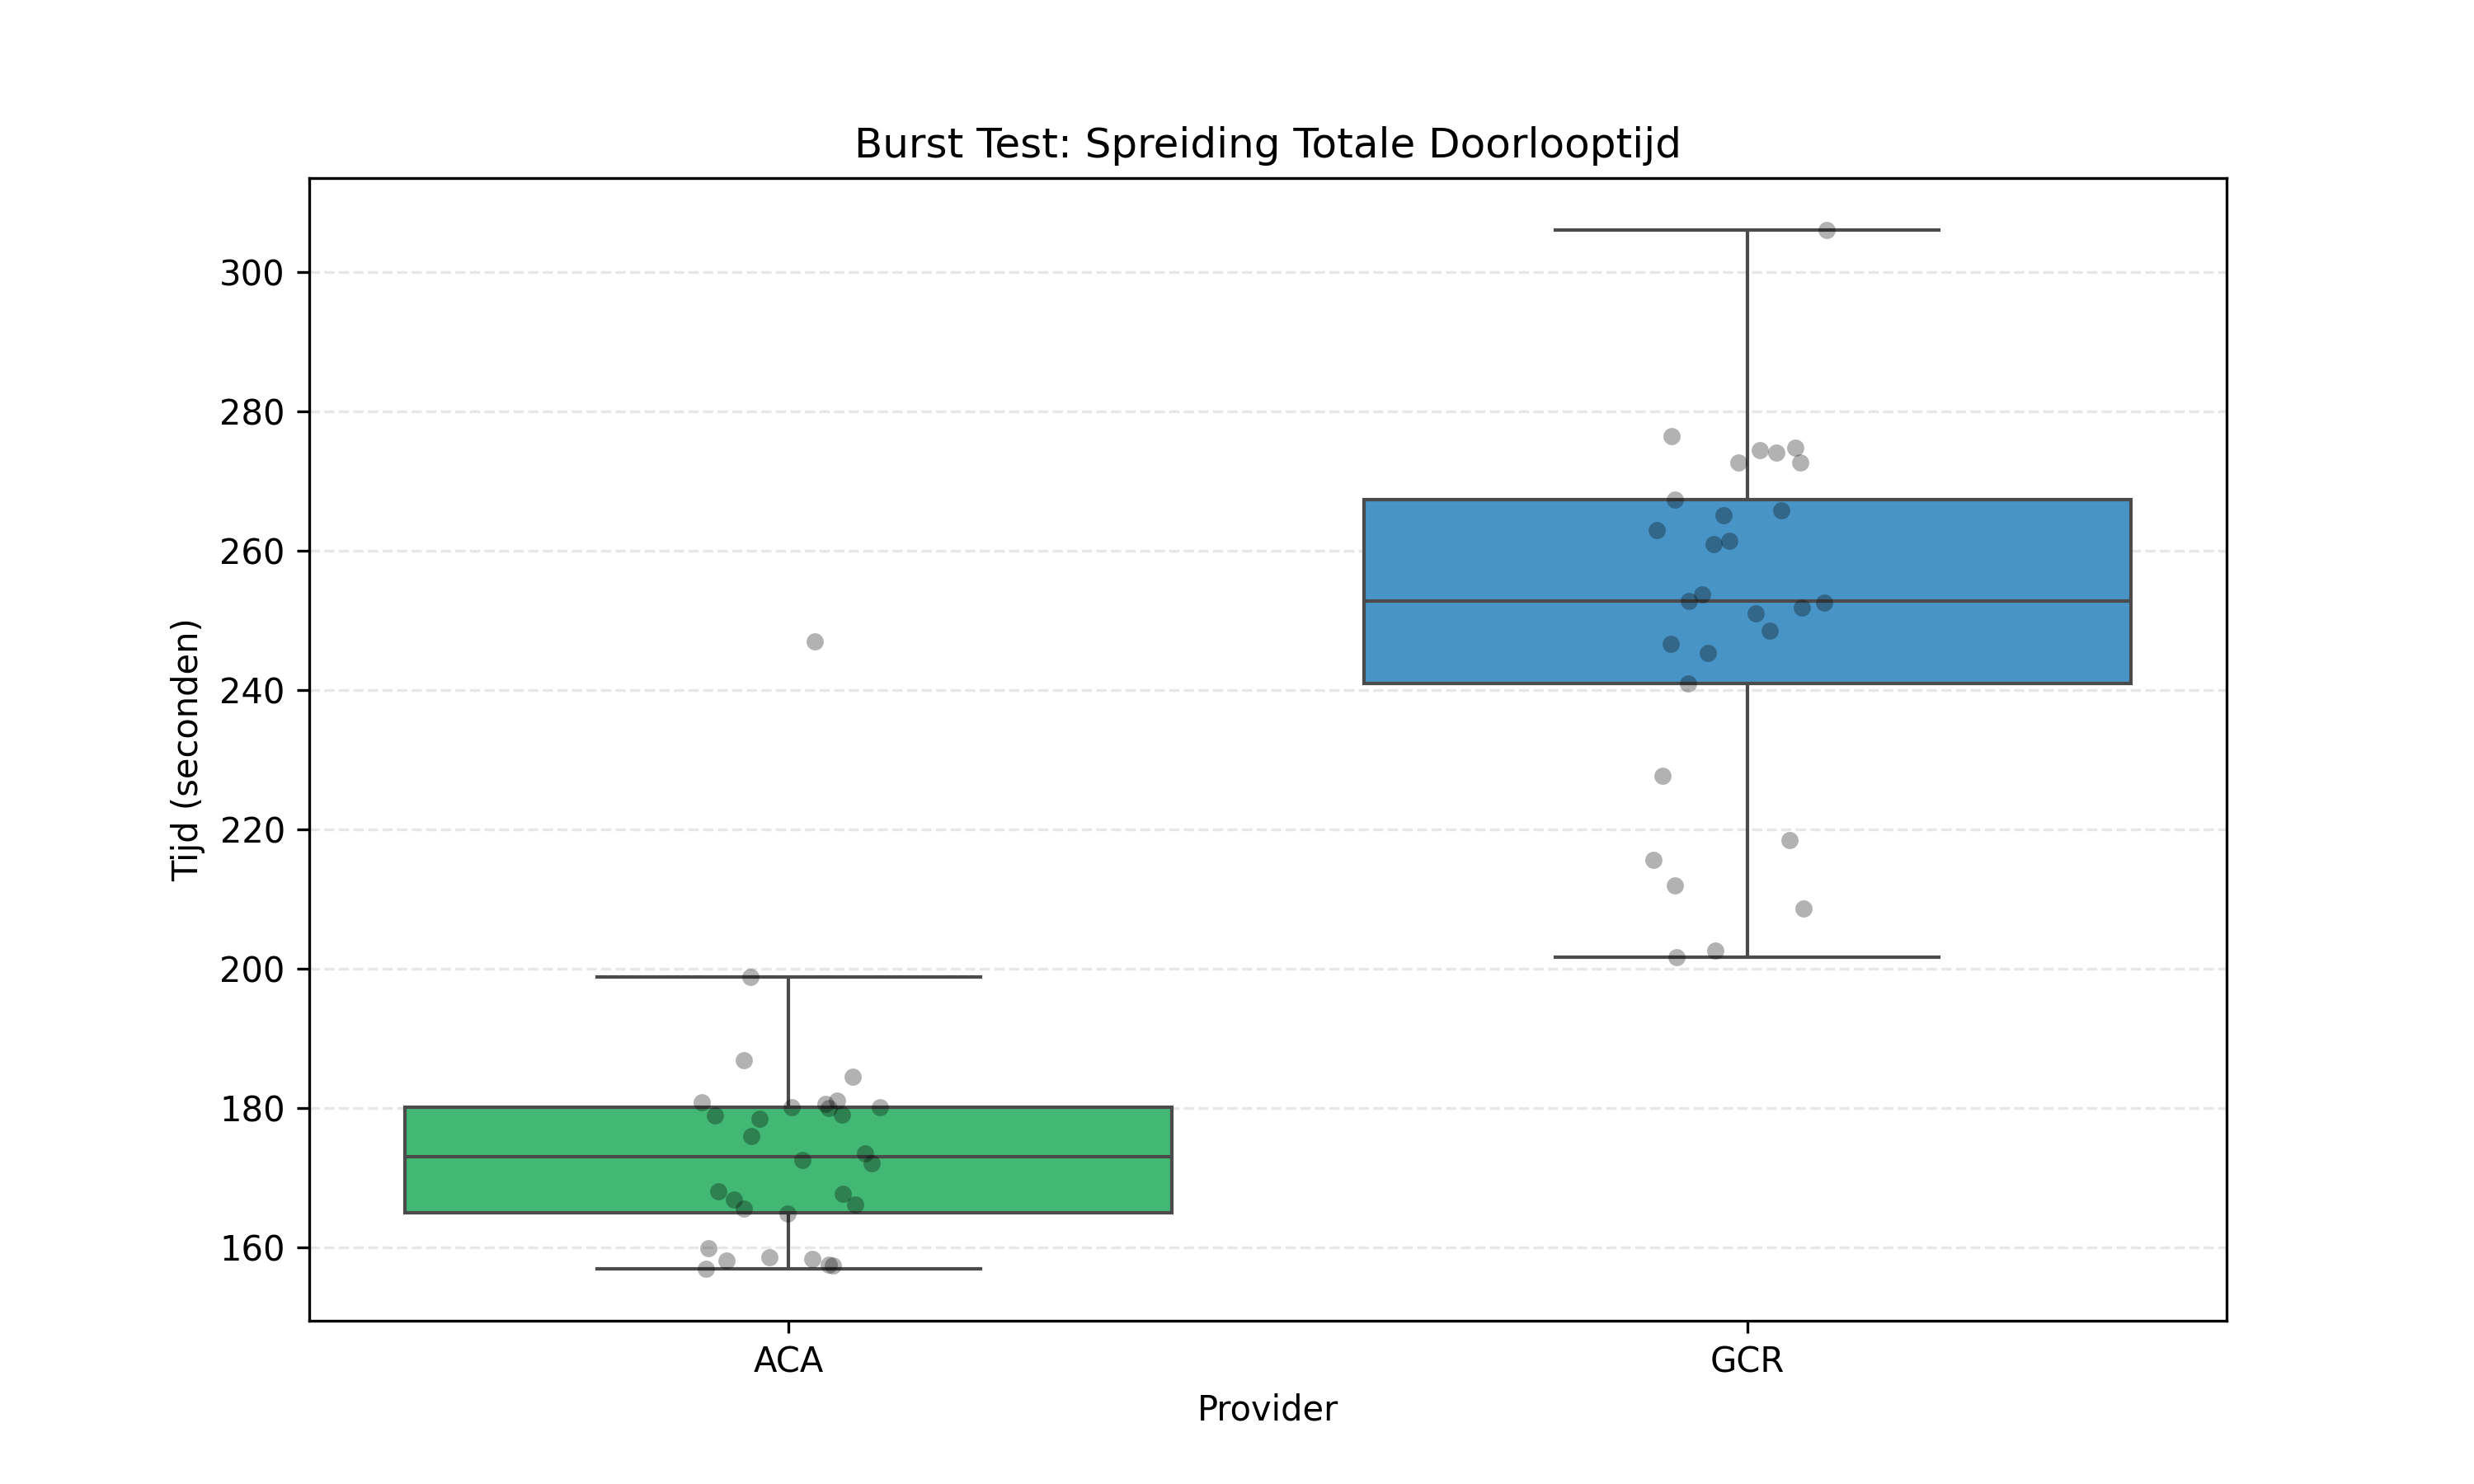
\includegraphics[width=\textwidth]{../graphics/burst_boxplot_spreiding.png}
    \caption{Burst: Spreiding totale doorlooptijd}
\end{figure}

De boxplot toont duidelijk het verschil tussen ACA en GCR. De spreiding bij GCR is veel groter en de doorlooptijd is ook gemiddeld hoger. Ondanks de toenemende druk lijkt ACA de superieure oplossing te zijn in deze context.

\subsection{Totale Doorlooptijd}

\begin{figure}[H]
    \centering
    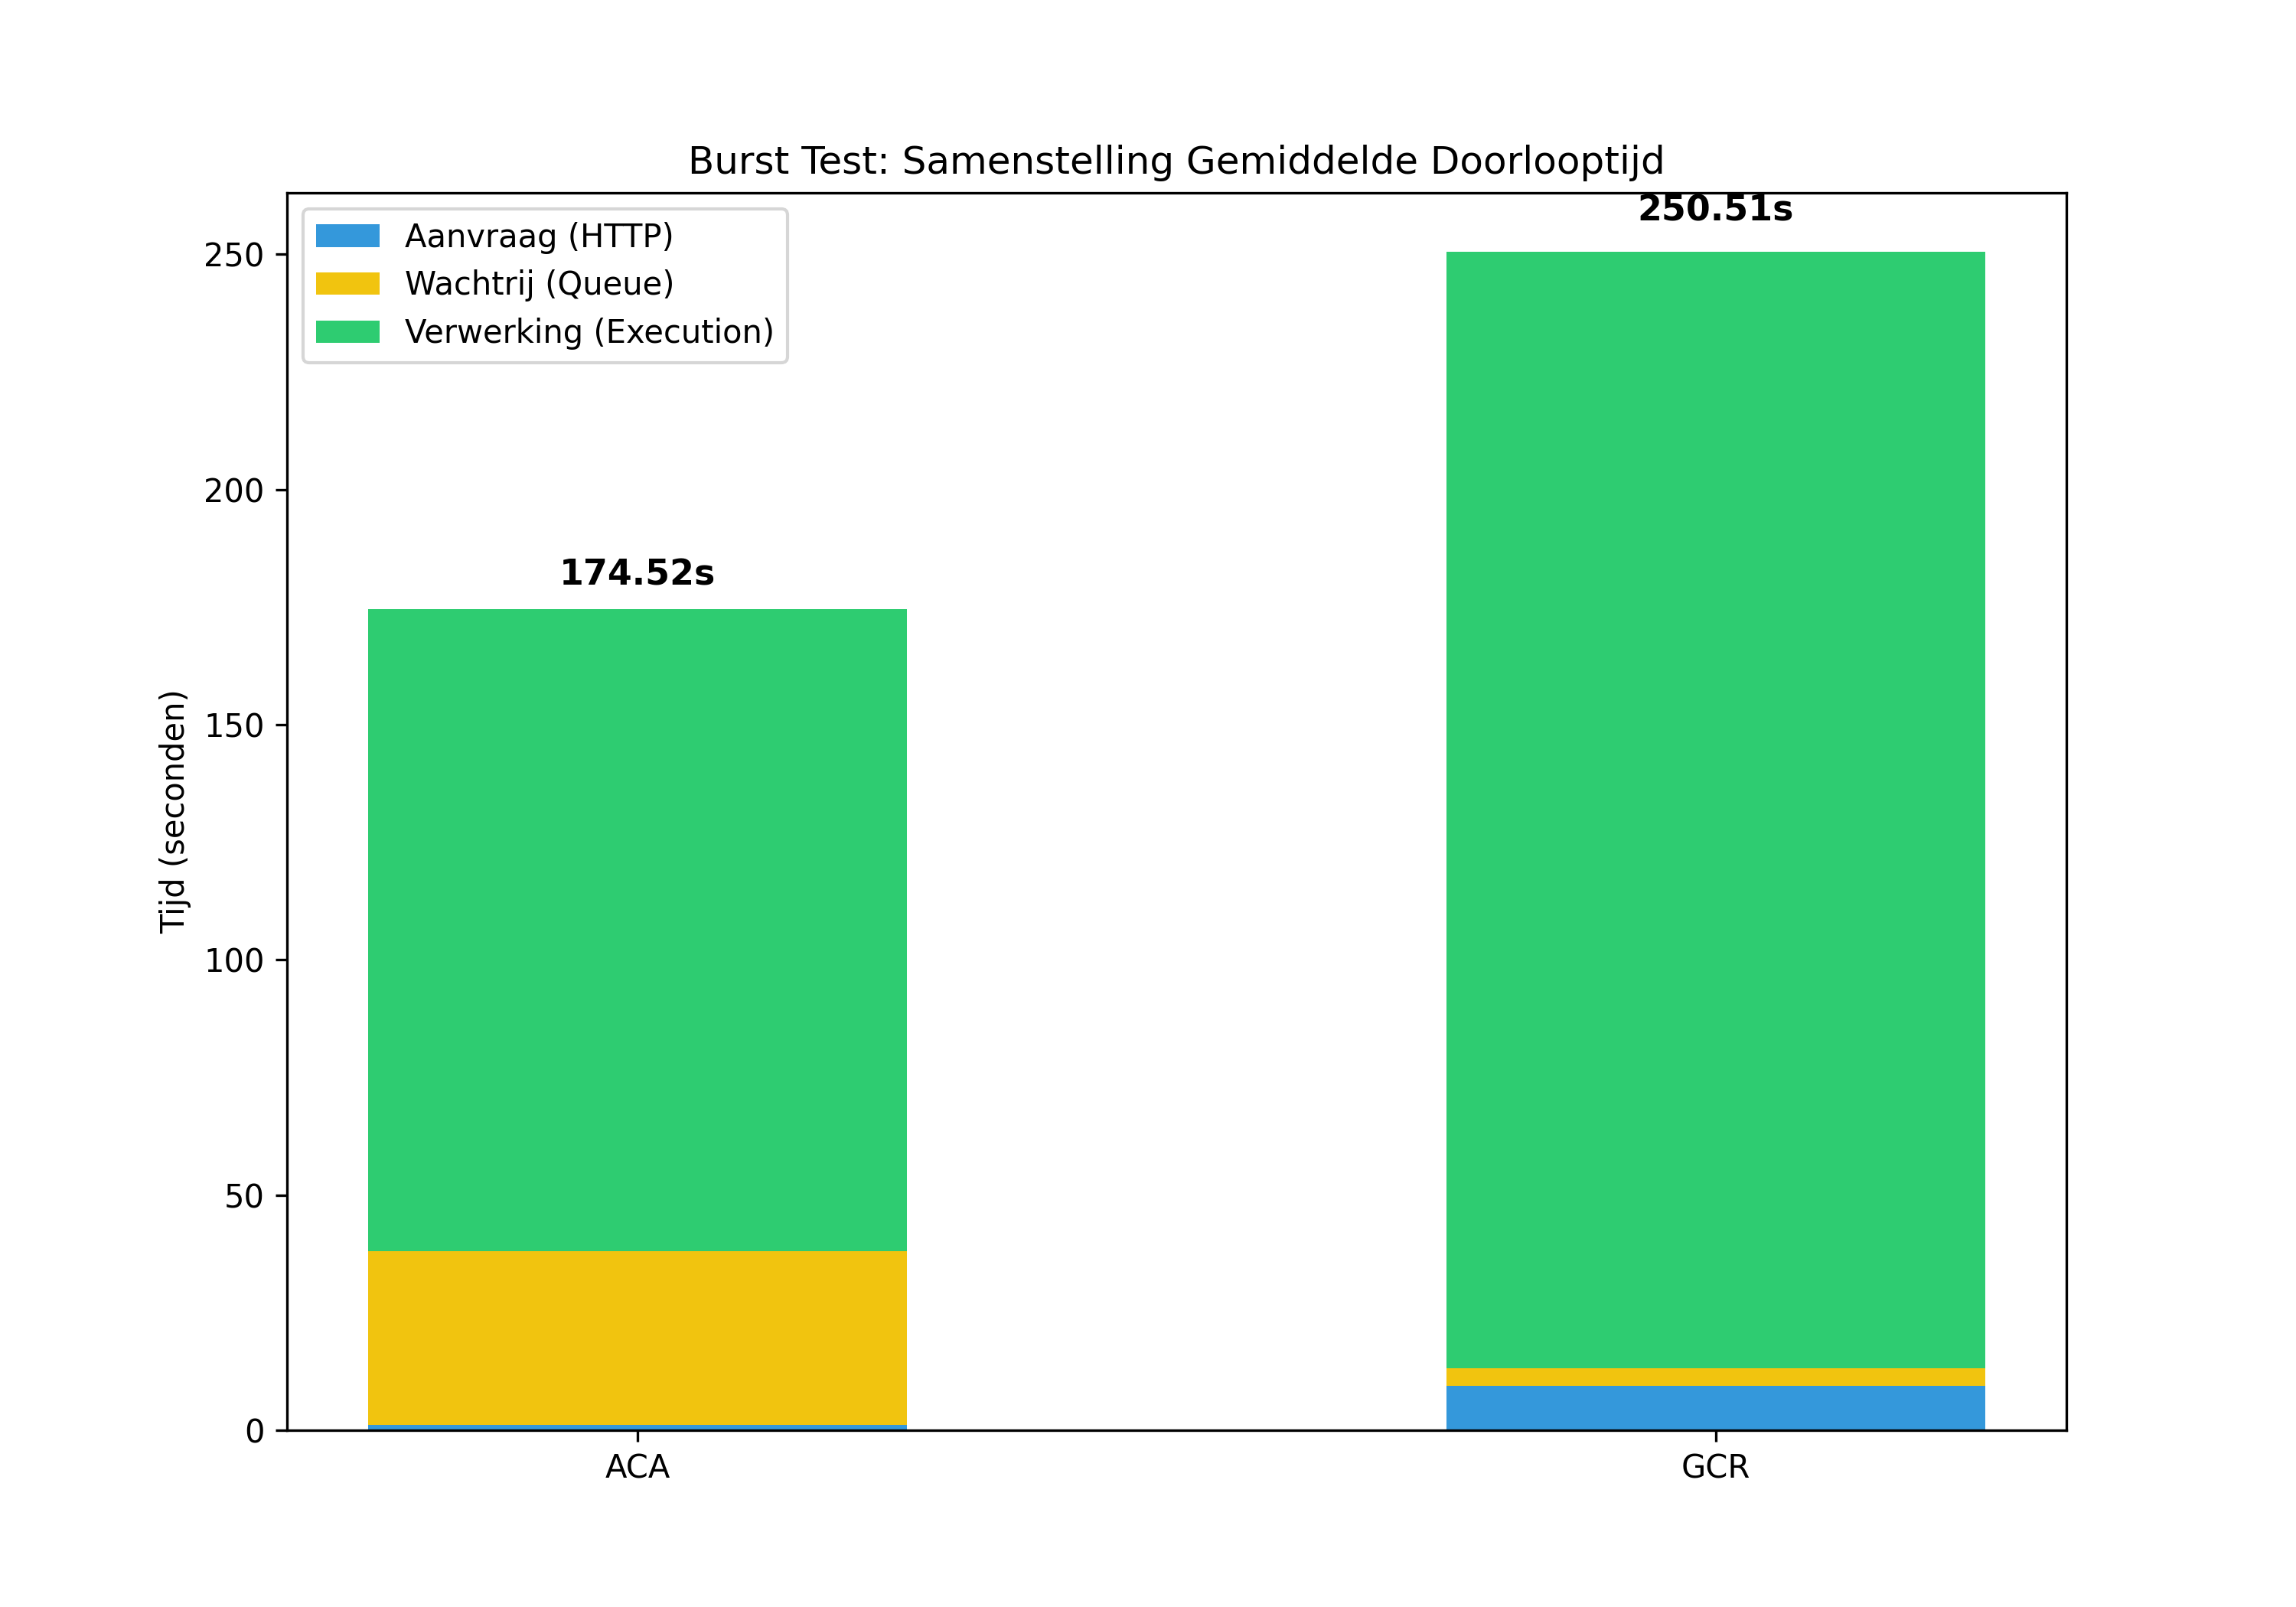
\includegraphics[width=\textwidth]{../graphics/burst_stacked_doorlooptijd.png}
    \caption{Burst: Gemiddelde Doorlooptijd}
\end{figure}

Deze grafiek visualiseert dat de wachtrij bij ACA volloopt en gemiddeld langer duurt om een container toe te wijzen aan een job. Bij GCR lijkt de aanvraagtijd langer te duren dan bij ACA, maar is de wachtrijverwerking wel veel efficiënter.

\section{Geheugenefficiëntie}

\subsection{Burst}

\begin{figure}[H]
    \centering
    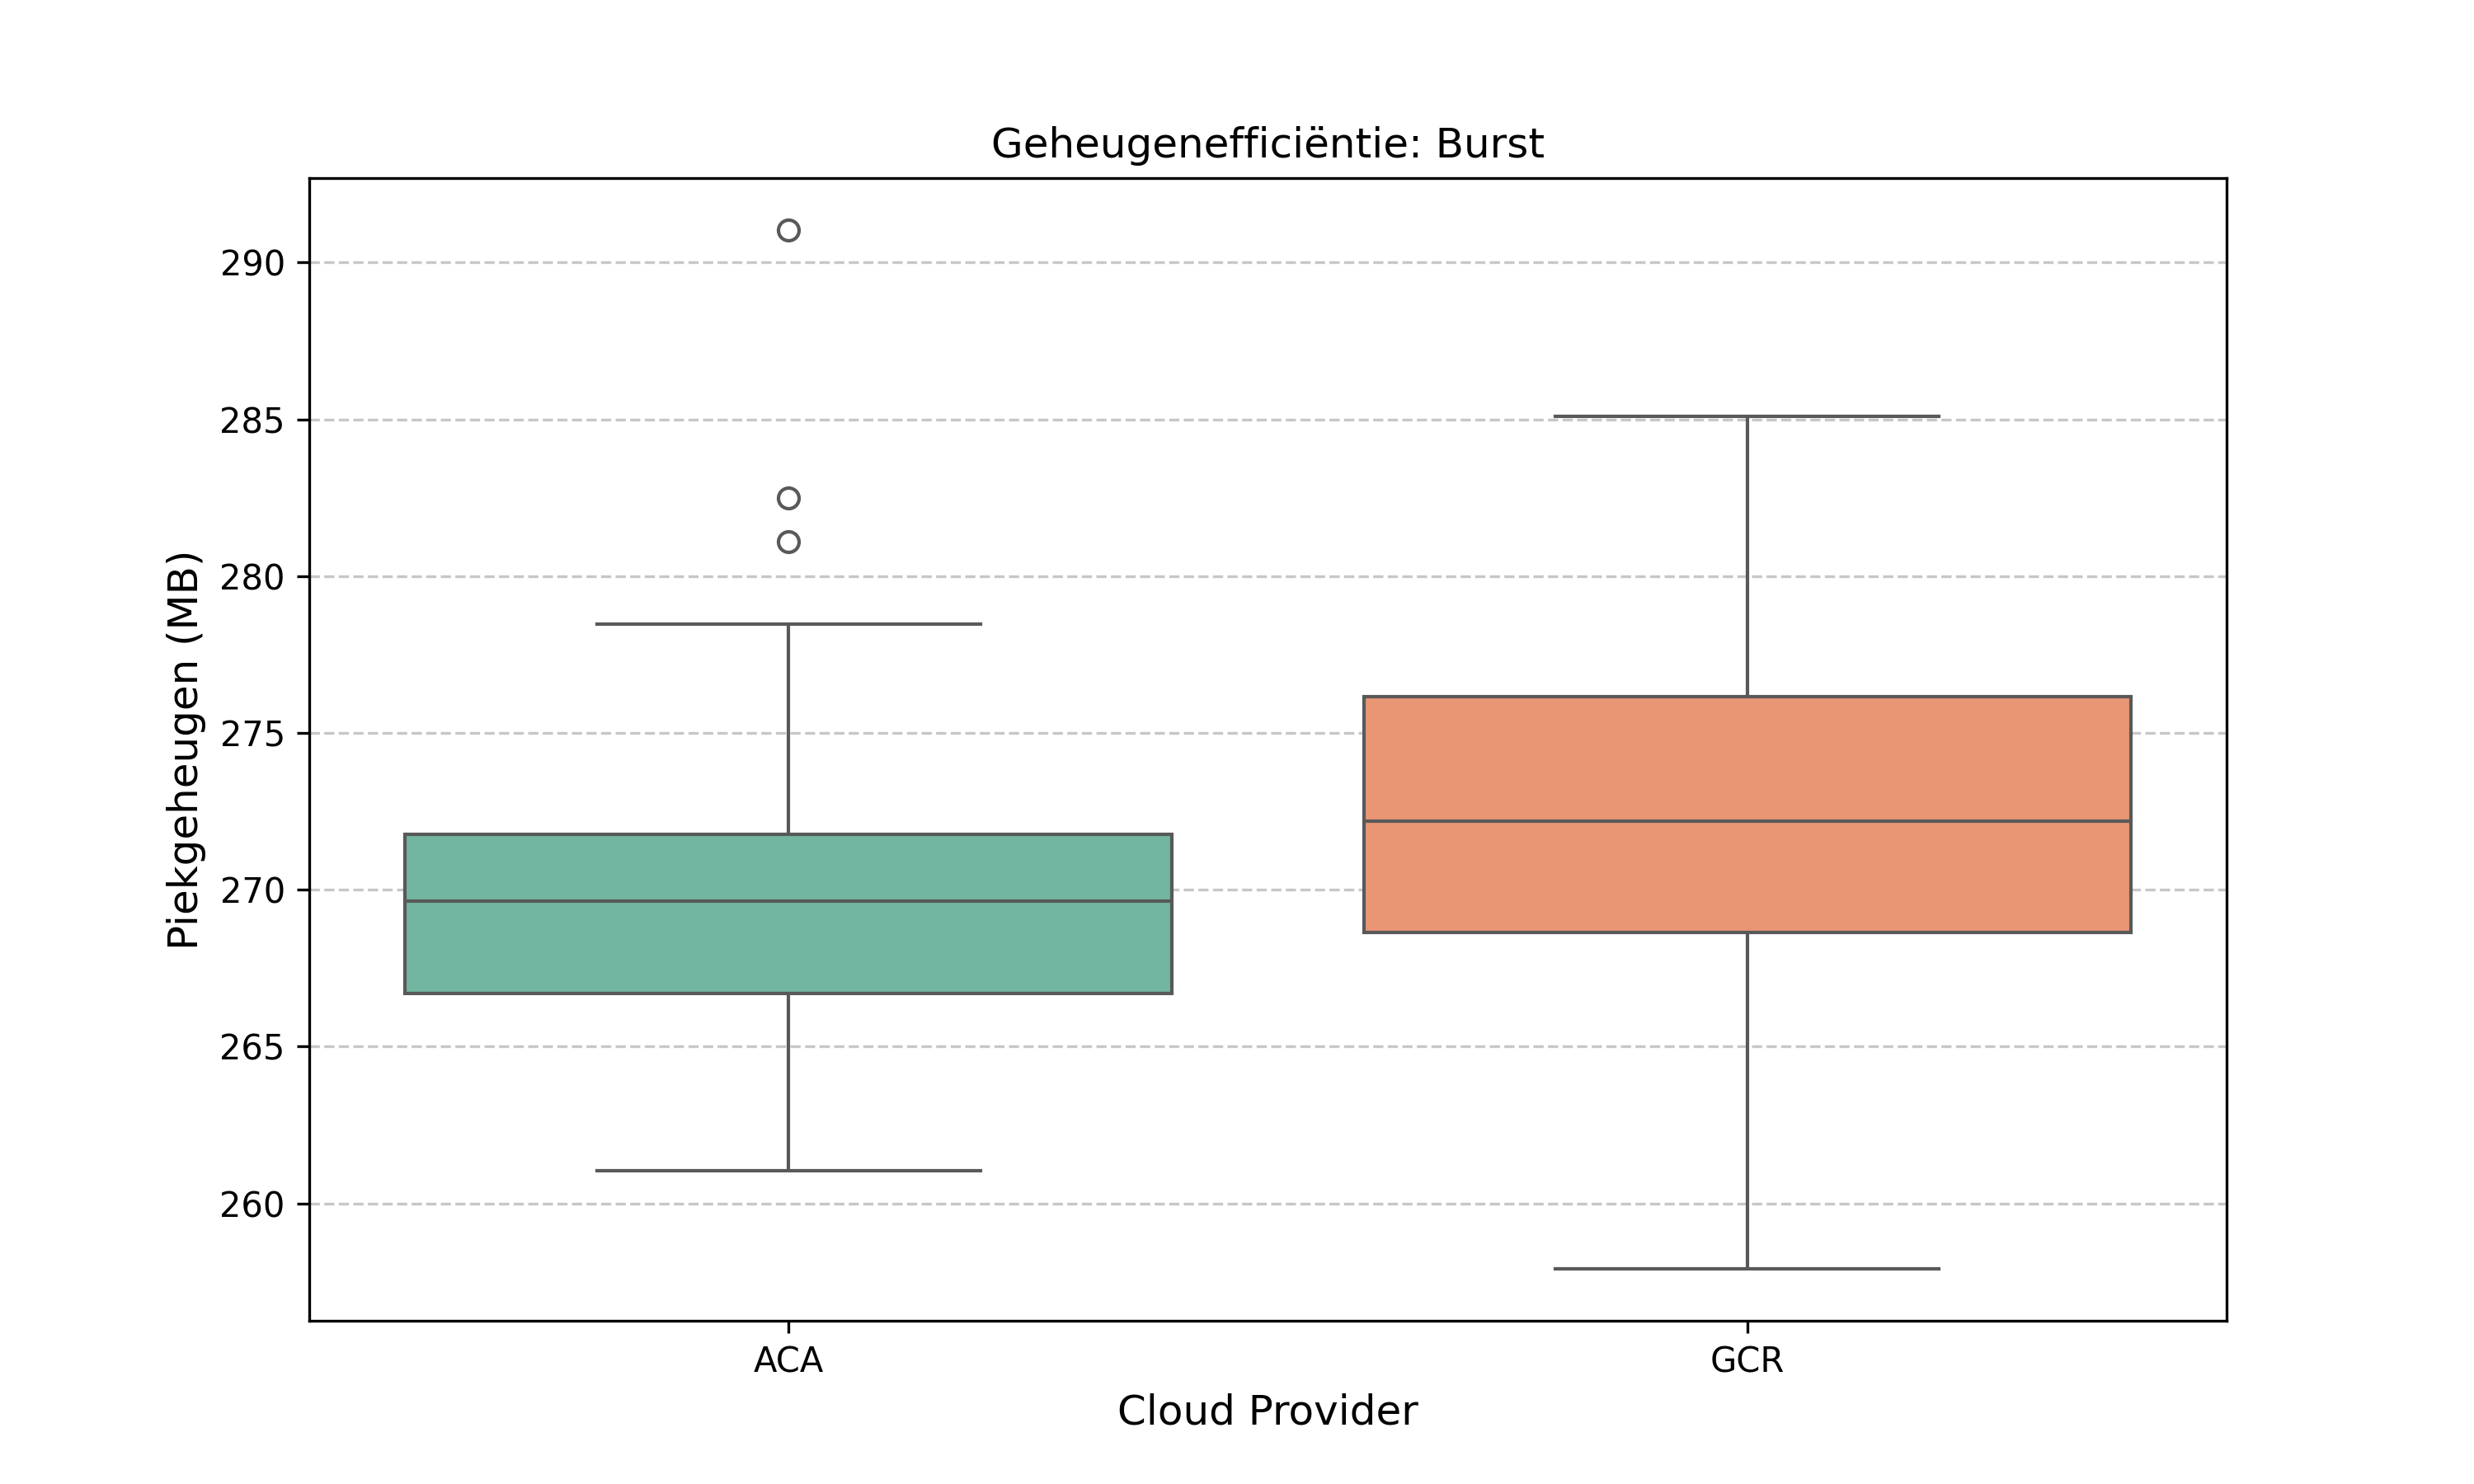
\includegraphics[width=\textwidth]{../graphics/geheugenefficientie_burst.png}
    \caption{Geheugenefficiëntie: Burst}
\end{figure}

\subsubsection{Hypothese H9} 

\begin{description}
    \item[Stelling:] Er is geen significant verschil in het piekgeheugengebruik tussen GCR en ACA voor identieke taken bij een burst.
    \item[Resultaat:] Behouden ($p = 0,065$)
\end{description}

Beide cloud-omgevingen gebruiken de toegewezen resources even efficiënt bij de verwerking. Er is statistisch geen beduidend verschil tussen GCR (272MB) en ACA (270MB) bij een piekbelasting.

\subsection{Warm vs Burst}

\begin{figure}[H]
    \centering
    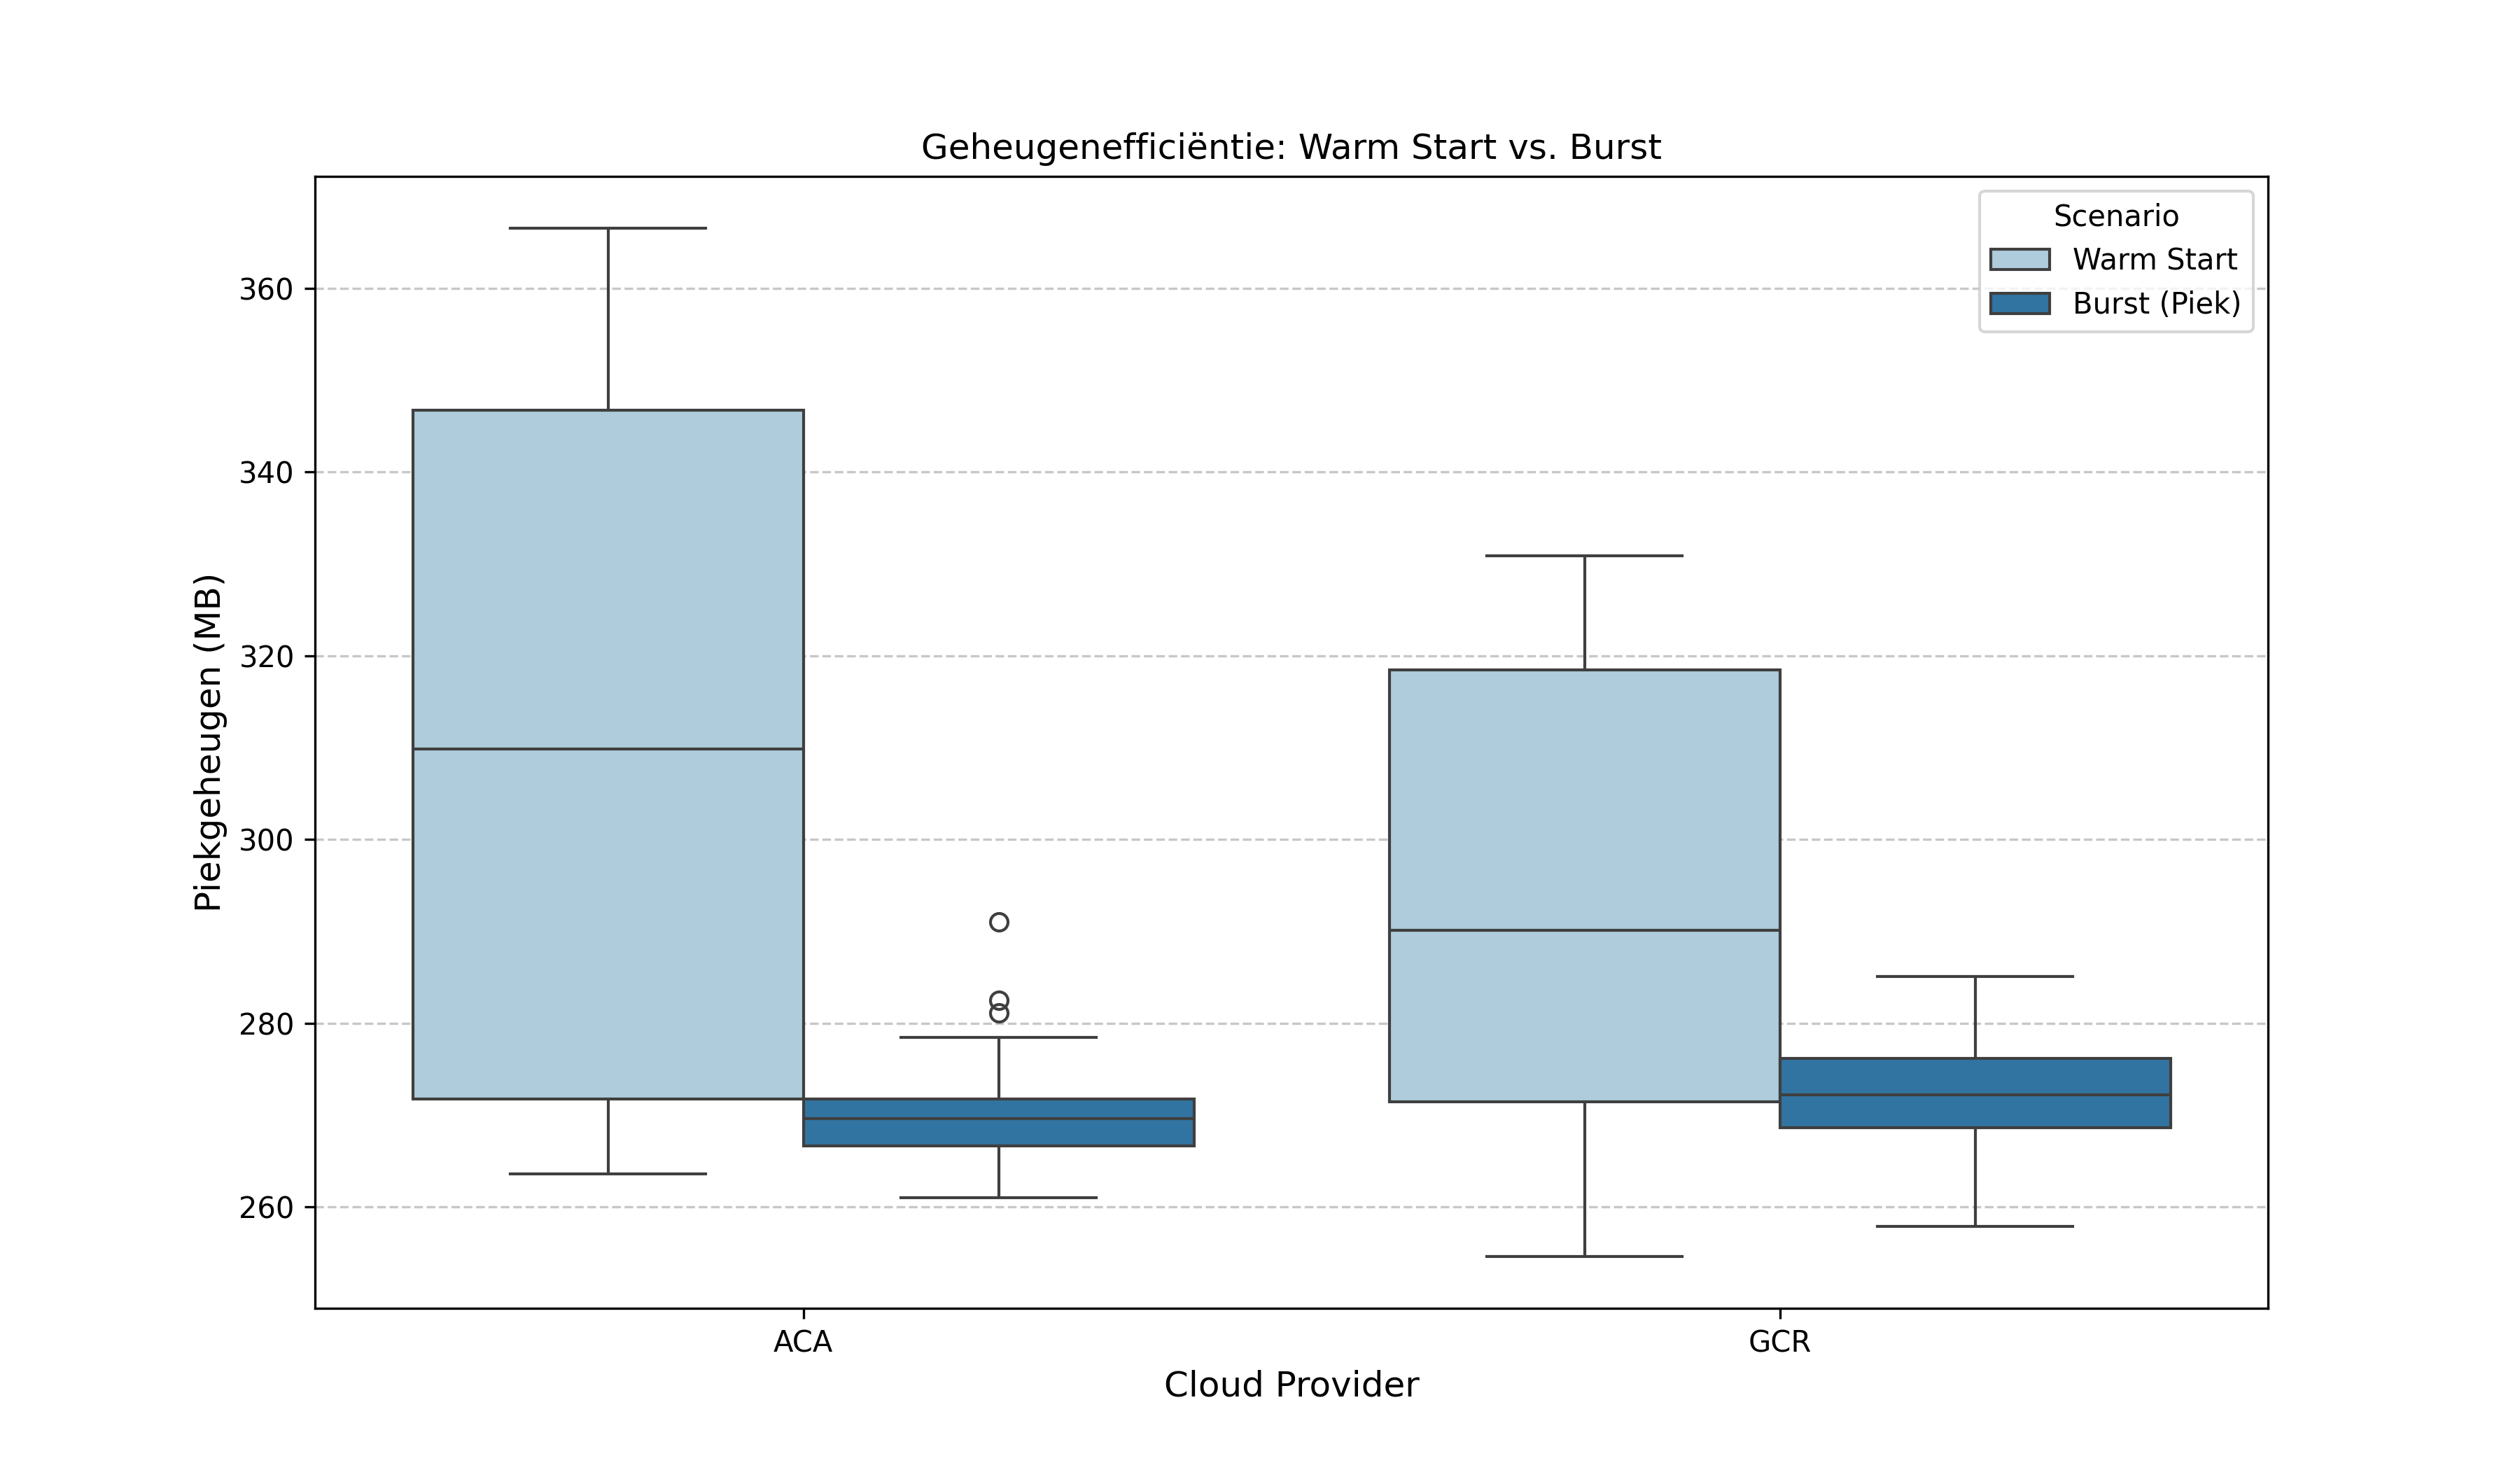
\includegraphics[width=\textwidth]{../graphics/geheugenefficientie_warm_burst.png}
    \caption{Geheugenefficiëntie: Warm Start vs. Burst}
\end{figure}

\subsubsection{Hypothese H10} 

\begin{description}
    \item[Stelling:] Het piekgeheugengebruik van de containers blijft constant, ongeacht of het een warme start of een burst betreft.
    \item[Resultaat:] Verworpen ($p < 0,001$)
\end{description}

Het piekgeheugen is opvallend hoger bij de warme start dan bij de burst voor beide omgevingen. Dit wordt ook aangegeven in de statistische toetsing. Beide oplossingen worden verplicht om bij een piekbelasting efficiënter om te gaan met de resources om te voorkomen dat ze vastlopen bij de verwerking. De grafiek geeft visueel mee dat de sprong bij ACA tussen beide situaties groter is dan bij GCR. ACA gaat naar gemiddeld minder piekgeheugen (ontktacht bij H9) bij burst naar gemiddeld meer piekgeheugen bij warme start ten opzichte van GCR.  

\section{Kostenraming}

Dit onderdeel schat de nodige kosten in om een totale overgang naar de nieuwe omgevingen te realiseren. De kosten worden opgesplitst in 2 onderverdelingen:

\begin{enumerate}
    \item Eénmalige kosten die noodzakelijk zijn om de huidige toepassing te moderniseren, container-klaar te maken en om de cloud-omgeving op te zetten.
    \item Vaste maandelijkse kosten die afhankelijk zijn van verschillende componenten die elk hun eigen prijs hebben per maand. 
\end{enumerate}

\subsection{Migratie-kosten}

Het uurloon van de programmeur die deze migratie zal uitvoeren, wordt in de berekeningen op €50 geschat.

\begin{table}[H]
    \centering
    \caption{Eénmalige kost per omgeving}
    \label{tab:vaste-kost}
    \begin{tabular}{|l|l|l|}
        \hline
        \textbf{Categorie} & \textbf{Azure Container App} & \textbf{Google Cloud Run} \\ \hline
        Analyse & €100 (2u x €50) & €100 (2u x €50) \\ \hline
        Refactoring & €1000 (20u x €50) & €1000 (20u x €50) \\ \hline
        Containerisatie & €100 (2u x €50) & €100 (2u x €50) \\ \hline
        Infrastructuur \& Beveiliging & €400 (8u x €50) & €600 (12u x €50) \\ \hline
        CI/CD & €300 (6u x €50) & €300 (6u x €50) \\ \hline
        Testen en Finetuning & €200 (4u x €50) & €200 (4u x €50) \\ \hline \hline
        \textbf{Totaal} & \textbf{€2100 (42u x €50)} & \textbf{€2300 (46u x €50)} \\ \hline
    \end{tabular}
\end{table}

\begin{description}
    \item[Analyse] 
    Er dient een kleine analyse uitgevoerd te worden van deze Proof-of-Concept en de impact op de bestaande toepassing. 
    \item [Refactoring] 
    De huidige code moet omgezet worden van .NET Core 3.1 naar .NET 8 Isolated Worker. Dit heeft impact op de libraries en dependencies die ook geüpdatet moeten worden. Anderzijds zijn er ook aanpassingen nodig in de architectuur en lifecycle managment van de objecten in het programma.
    \item[Containerisatie] 
    Er moet een Dockerfile opgesteld worden die zal dienen om de structuur van de container te definiëren.
    \item[Infrastructuur \& Beveiliging]
    De service wordt opgezet in Azure Container Apps of Google Cloud Run. Er moet ook gekeken worden naar de beveiliging van deze opzet, zodat het beschermd is op productie. De tijd om de opzet te realiseren in beide omgevingen wordt als  evenredig ingeschat. Het verschil in tijd bevindt zich bij de beveiliging, aangezien GCR cross-platform moet werken en ACA niet, moet er meer tijd voorzien worden voor GCR.
    \item[CI/CD]
    Dit bevat een Registry Setup die de image van de container zal beheren, alsook de beveiliging om te bepalen wie de image mag pushen en pullen. Verder moet er een \textit{Build} en \textit{Release} Pipeline opgezet worden en moet er rekening gehouden worden met \textit{Secret Management}.
    \item[Testen en Finetuning] 
    Deze tijd moet voorzien worden om de nieuwe applicatie tot in de puntjes klaar te hebben. Het dient ook als buffertijd voor onvoorziene omstandigheden.
\end{description}

\subsection{Vaste Maandelijkse Kosten}

Om de maandelijkse kosten in te schatten wordt er vanuit gegaan dat de applicatie 1000 aanvragen per maand krijgt. Om te bepalen hoeveel actieve verwerkingstijd er in rekening gebracht wordt, werd er een optelling gedaan van het verschil tussen de start- en stoptijd van de HttpTrigger en de start- en stoptijd van de achtergrondverwerking per provider voor resultaten van de warm start testcase. Een maand wordt in dit overzicht aanzien als een maand van 31 dagen.

\begin{table}[H]
    \centering
    \caption{Vaste maandelijkse kosten per omgeving voor 1000 aanvragen}
    \label{tab:maandelijkse-kost}
    \begin{tabular}{|l|l|l|}
        \hline
        \textbf{Categorie} & \textbf{Azure Container App} & \textbf{Google Cloud Run} \\ \hline
        Aanvragen & €0,00 (Free tier) & €0,00 (Free tier) \\ \hline
        CPU & €0,00 (Free tier) & €1,97 (Net boven free tier) \\ \hline
        Geheugen & €0,00 (Free tier) & €0,41 (Net boven free tier) \\ \hline
        Netwerk (Egress) & €0,00 (Free tier) & €1,44 (16 GiB x €0,09) \\ \hline
        Image Beheer & €4,41 (Vast tarief) & €0,00 (Free tier) \\ \hline
        Message Broker & €0,01 (Service Bus) & €0,00 (Pub/Sub free tier) \\ \hline
        CI/CD & €0,00 (Free tier) & €0,00 (Free tier) \\ \hline
        Secret Manager & €0,00 (Free tier) & €0,00 (Free tier) \\ \hline
        Beveiliging & €0,00 (Free tier) & €0,00 (Free tier) \\ \hline
        Observability & €0,00 (Free tier) & €0,00 (Free tier) \\ \hline \hline
        \textbf{Totaal} & \textbf{€4,42} & \textbf{€3,82} \\ \hline
    \end{tabular}
\end{table}

\begin{description}
    \item[Aanvragen, CPU \& Geheugen]
    Dit is de directe rekenkracht die nodig is voor het genereren van de dataset. Bij ACA vallen deze kosten bij 1000 aanvragen volledig binnen de maandelijkse \textit{free grants}. GCR gaat licht over de gratis drempel voor actieve verwerkingstijd, wat resulteert in een kleine kost voor CPU en geheugen.
    \item[Netwerk (Egress)]
    Dit Vertegenwoordigt de kosten voor data die de cloud-omgeving verlaat. Bij ACA blijft dit verkeer binnen dezelfde regio en is het kosteloos. Bij GCR wordt de data verzonden naar de Azure-omgeving van Agromanager, waarvoor een tarief per GiB aangerekend wordt.
    \item[Image Beheer]
    Dit regelt de opslag van de container-images. Azure rekent een vast dagtarief voor de Azure Container Registry aan. Google Cloud factureert op basis van het werkelijke verbruik in de Artifact Registry, wat voor de huidige image-omvang (503 MiB) binnen de \textit{free tier} valt.
    \item[Message Broker]
    Het component dat de asynchrone communicatie tussen de HttpTrigger en de achtergrondverwerking beheert. Beide providers bieden een ruime gratis quota aan. bij Azure is een minimale kost van €0,01t opgenomen voor de Service Bus-operaties.
    \item[Overige componenten]
    Diensten voor CI/CD, Secret Management, Beveiliging en Observability zijn essentieel voor de productie-omgeving. Voor  1000 aanvragen per maand vallen de gebruikskosten van deze diensten bij beide providers volledig binnen de beschikbare \textit{free tiers}.
\end{description}